\documentclass[10pt]{article}
% MAXIMUM VIEWER COMPATIBILITY. pdfTeX writes PDF 1.5 by default, which uses a
% compressed cross reference stream and object streams. Both are legal and both
% are what GitHub's in browser viewer most often fails to render, reporting the
% file as invalid when it is not. Dropping to 1.4 with object compression off
% writes a classic xref table, which every viewer reads. It costs some file size
% and nothing else.
\pdfminorversion=4
\pdfobjcompresslevel=0
\pdfcompresslevel=9

\usepackage[margin=1in]{geometry}
\usepackage{amsmath,amssymb}
\usepackage{booktabs}
\usepackage{graphicx}
\usepackage{array}
\usepackage{rotating}% Table 6 on a landscape page (review item 15)
\usepackage[hidelinks]{hyperref}
\expandafter\def\expandafter\UrlBreaks\expandafter{\UrlBreaks\do-}% long URLs may break at a hyphen
\usepackage{xcolor}
% colour carried across a page break inside a footnote leaked into the body (2 October: Section 6 printed red)
\usepackage{pdfcolfoot}
% Everything revised in this draft is marked in red: the move to two periods and
% the responses to the comments on the previous version. The change of
% terminology from "the disorder" to "a SUD" runs through the whole note and is
% NOT marked, since colouring every instance would colour half the document.
% fill.py wraps in every number that MOVED against numbers_prev.json, so
% the note marks a changed number automatically rather than by hand. Set it to red
% so a recalibration shows up as red without anyone having to find the numbers.
% To clear the marks, copy the current numbers over numbers_prev.json and refill.
% is the mark fill.py puts on every number that moved since
% numbers_prev.json. It prints as ordinary text: the reader asked not to see the
% pipeline's own bookkeeping in red. The mark survives in the generated .tex,
% so grepping the generated file for the macro finds what moved, and grepping
% .src.tex for the at signs finds every number the stylized pipeline still
% supplies and the quantitative model has yet to replace.
% \textcolor is NOT \long: a red span that crossed a blank line died with
% "Paragraph ended before \@textcolor was complete", and pdflatex then
% returned nonzero, which set -e turned into a build that stopped before
% every checker in build.sh. \color is a switch and survives \par.
% \new MUST RENDER RED. strip_red.py rewrites this line to a passthrough,
% \newcommand{\new}[1]{#1}, so that any \new left after a strip is inert.
% That passthrough was committed once and every \new written afterwards
% went in as plain black text: several rounds of marked edits were
% invisible to the reader, in the intro, the calibration entries and the
% citations alike, while table cells kept showing red because they use
% \textcolor directly. check_red.py now fails the build if this line is
% a passthrough while any \new remains in the file.
\newcommand{\new}[1]{{\color{red}#1}}
% DELETIONS STRUCK THROUGH (the author, 11 October: "if you delete something i want to see what you deleted"):
% \del prints what a round took out, red and struck; writing/tools/track_changes.py writes it, strip_red.py removes it.
\DeclareRobustCommand{\del}[1]{\sout{#1}}
% WHAT THE NEXT SIMULATIONS CHANGE (2 October): \upd tags a paragraph or a sentence, \updnum colours a number or a
% generated sentence that will be refilled. Blue, so they are never confused with the red of an edit; the red
% strippers leave them alone, and each goes when its paragraph is rewritten from the new runs.
\usepackage{marginnote}
% each \upd also flags the margin (marginnote works in minipages and floats, where \marginpar does not) and
% enters the list printed after the abstract, with its page, so every pending update can be found and clicked to
% HIDDEN IN THE PDF (the author, 6 October: "remove the blue I see in the pdf but keep placeholders for yourself for
% things you need to check/update"). The \upd tags and \updnum marks stay in the source as the list of what the next
% simulations refresh -- grep for them -- but print nothing (\upd, \listofupdates) or plain black (\updnum) while
% \showupdatesfalse. Set \showupdatestrue to see them in blue again.
\newif\ifshowupdates \showupdatesfalse
\newcommand{\upd}[1]{\ifshowupdates\phantomsection\addcontentsline{upd}{subsection}{#1}%
  \marginnote{\color{blue}\textbf{UPDATE}}{\color{blue}\textbf{[UPDATE: #1]}}\fi\ignorespaces}
\makeatletter
\newcommand{\listofupdates}{\ifshowupdates\par\noindent{\color{blue}\textbf{Pending updates from the new simulations}}\par
  {\small\@starttoc{upd}}\fi}
\makeatother
\newcommand{\updnum}[1]{\ifshowupdates{\color{blue}#1}\else#1\fi}
% WHAT A ROUND DELETED, AND WHY IT CHANGED (the author, 3 October: "deleted sentences should show as crossed so I
% know what you delete", and "leave notes for me in case I need to understand why you made a change"). \del prints
% deleted text struck through in red; \why prints a note in green and lists it, with its page, after the abstract.
% Both go, contents and all, when red is stripped (writing/tools/marks.py), and the checkers do not read them.
\usepackage[normalem]{ulem}
% \tocheck{...} HIGHLIGHTS A CLAIM STILL TO BE VERIFIED (the author, 9 October: "we need to verify if this is the
% reason or the drug price. please highlight it"): yellow in the PDF until the run that settles it is in
\usepackage{soul}\sethlcolor{yellow}
\usepackage{placeins} % \FloatBarrier before the transition: Tables 5 and 6 stay with the long run (the author, 11 October)
\newcommand{\tocheck}[1]{\hl{#1}}
\soulregister{\updnum}{1} % soul passes the blue transition numbers through the yellow highlight
\soulregister{\ref}{7} % and a cross-reference, whole (round r322: the transition's text is yellow)
% \ai{...} MARKS A SENTENCE AN AI DETECTOR FLAGGED (the author, 20 October: "almost all the previous sentences are
% still highlighted by the AI detector", then "highlight for me the sentences, and ill try to write them myself"): blue
% until the author's own wording replaces it. Not a red mark, so strip_red.py leaves it.
\definecolor{aiblue}{rgb}{0.72,0.86,1}
\newcommand{\ai}[1]{{\sethlcolor{aiblue}\hl{#1}}}
\soulregister{\eqref}{7}
\DeclareRobustCommand{\del}[1]{\sout{#1}}
% a red pilcrow where a round starts a new paragraph (16 October); the strip removes it (writing/tools/marks.py)
\newcommand{\parmark}[1]{\P\ }
\definecolor{whygreen}{rgb}{0,0.45,0.2}
\newcommand{\why}[1]{\phantomsection\addcontentsline{why}{subsection}{#1}%
  {\color{whygreen}\footnotesize[Why: #1]}}
% \green{...}: text the author asked to keep in green (8 October, on the custody sentence: "keep in green").
% Not a red mark, so strip_red.py leaves it; it stays green until the author says otherwise.
\newcommand{\green}[1]{{\color{whygreen}#1}}
\makeatletter
\newcommand{\listofwhys}{\ifshowupdates\par\noindent{\color{whygreen}\textbf{Notes on this round's changes}}\par
  {\small\@starttoc{why}}\fi}
\makeatother
% A number not computed yet: a slot to fill, never a guess.
\newcommand{\blank}{\underline{\hspace{2.2em}}}
% A STANDING FLAG, which survives the strip between rounds. \new and \cut both
% mark what changed since the last version and are cleared when the next round
% starts, so neither can carry an open question forward. \query holds one: a
% short red note in the margin asking whether a passage should be there at all.
% It is not prose and must be gone before the note is circulated.
% A FLAG IS A FOOTNOTE, NOT A MARGIN NOTE, AND THAT IS NOT A STYLE CHOICE.
% As a \marginpar it broke float placement: the run reported "Float(s) lost",
% the standard parameters table was never placed, its \label went with it, and
% the three references to it printed as ??. That is the same ?? flagged in the
% margin two rounds ago and explained away then as a stale build; it was this.
% Rebuilt with \query made a no-op the run is clean, which is what identifies
% the cause. Blue, so a flag is never mistaken for a round's red.
\newcommand{\query}[1]{\footnote{\textcolor{blue}{#1}}}
% THE PARAMETER COUNTS AS MACROS, so the two table files can quote them too.
% fill.py only rewrites its placeholders in this file, and the tables are
% \input from
% their own .tex, so a caption saying how many rows its table has could not be
% generated any other way. Counted off the Set column of the tables themselves.
\newcommand{\nmain}{twenty-six}
\newcommand{\nstd}{thirty-three}
% The cut macro below marks a PROPOSED DELETION: red and struck through, so the reader sees what
% would go before it goes. ulem is not in this installation, and a single rule over a
% whole phrase cannot break across lines, so the rule is drawn word by word: each word
% is its own box and TeX breaks between them as usual. The scanner below splits the
% argument on spaces, which is why a cut must not contain a braced group with a space
% inside it. Maths is fine, $14.2$ is one word.
\makeatletter
\newlength{\cw@len}
\newcommand{\cw}[1]{{\settowidth{\cw@len}{#1}%
  \rlap{\textcolor{red}{\rule[0.55ex]{\cw@len}{0.4pt}}}\textcolor{red}{\hspace{0pt}#1}}}
\newcommand{\cut}[1]{\cut@scan#1 \@nil}
\def\cut@scan#1 #2\@nil{\cw{#1}\ifx\relax#2\relax\else\space\cut@scan#2\@nil\fi}
\makeatother
\usepackage[official]{eurosym}
\usepackage{longtable}
\usepackage{titlesec}

\setlength{\parskip}{0.18em}
\newcolumntype{L}[1]{>{\raggedright\arraybackslash}p{#1}}

\renewcommand{\topfraction}{0.92}
\renewcommand{\bottomfraction}{0.85}
\renewcommand{\textfraction}{0.06}
\renewcommand{\floatpagefraction}{0.80}
\setlength{\textfloatsep}{12pt plus 2pt minus 3pt}
\setlength{\intextsep}{10pt plus 2pt minus 3pt}

\newcommand{\notes}[2]{\par\vspace{0.4em}%
  \begin{minipage}{#1}\footnotesize #2\end{minipage}}
% A table's note should start and end exactly where the rules of the table do.
% \tabnote measures the table into a box first and sets the note to that width.
% Captions sit above the tables, and the default gap below one is small enough
% that the title touches the top rule. Set once so every table gets the same air.
\setlength{\belowcaptionskip}{0.6em}
\newsavebox{\ntbox}
\newcommand{\tabnote}[1]{\notes{\wd\ntbox}{#1}}
\titlespacing*{\subsection}{0pt}{1.4em plus 0.3em}{0.7em plus 0.15em}
\titlespacing*{\subsubsection}{0pt}{1.1em plus 0.25em}{0.6em plus 0.15em}

\begin{document}

\begin{center}
\renewcommand{\thefootnote}{\fnsymbol{footnote}}
{\Large\bfseries Housing First or Treatment First? Ask the Kids, Not the Parents}\footnote{I thank Ay\c{s}e \.{I}mrohoro\u{g}lu, Kai Zhao, Joseph Steinberg, Efraim Benmelech, Jonathan Alschech, Ryan Quandt, Christopher Sharp and the seminar participants at the University of Toronto for their helpful comments. The data and replication code are available on GitHub at \url{https://github.com/srotberg/housing_first_or_treatment_first_ask_the_kids_not_the_parents}.}\\[0.6em]
{\large Shahar Rotberg}\footnote{Canada Mortgage and Housing Corporation (CMHC). Contact: \url{shahar.rotberg@gmail.com}. Website: \url{www.shaharrotberg.com}. This work was conducted on personal equipment and time, was not funded by any person or entity, and the author was not influenced by anyone at any point in this research. The author owns the code; he wrote the baseline code of the quantitative model. Claude (Anthropic) was used to write the code of the stylized model and extensions of the quantitative model, to debug the code, and to run the simulations. Every number in the paper is generated from that code, the two models were checked against each other on every mechanism they share, with the discrepancies found and their resolution logged in the replication package, and the code is public. The opinions expressed herein do not necessarily represent the views of CMHC.}\\[0.35em]
\today
\end{center}
\renewcommand{\thefootnote}{\arabic{footnote}}
\setcounter{footnote}{0}

\vspace{0.4em}
\begin{center}
\begin{minipage}{0.86\textwidth}
\begin{center}\textbf{Abstract}\end{center}
\noindent Should housing assistance require sobriety? A general-equilibrium model of homelessness, drug use, drug prices and mortality is calibrated to US data. Use concentrates among low-income households because a substance use disorder's mortality risk, unlike its unemployment risk, is uninsurable. Drug use harms users' children, cutting their consumption and, through a parent's disorder, their adult earnings. In the long run, sobriety conditions reduce these harms and, in aggregate, also childhood homelessness. Consequently, a newborn's welfare rises by $2.57$ percent of lifetime consumption, of which three quarters is an externality its parent does not count, and in general equilibrium parents gain too. Even along the transition, homelessness and childhood homelessness do not rise, and newborns still gain. The model reproduces micro evidence of randomised controlled trials, and users with a disorder lose, but macro effects on other households and children overturn the verdict. Moral hazard alone does not justify conditionality.

\vspace{0.6em}
\noindent\textit{Keywords:} homelessness; housing vouchers; substance
use disorder; intergenerational spillovers; externalities.

\vspace{0.2em}
\noindent\textit{JEL classification:} I18; I38; H23; R21; J62.
\end{minipage}
\end{center}

\vspace{0.8em}


%======================================================================
\listofupdates

\listofwhys

\section{Introduction}\label{sec:intro}

According to the point-in-time (PiT) count of January 2024 performed by the Department of Housing and Urban Development (HUD), at least $771{,}480$ people were sleeping in shelters or on the street, the most since the count began. In July 2025 an executive order directed the federal agencies to end support for Housing First policies that, in its words, ``fail to promote treatment, recovery, and self-sufficiency''.\footnote{Executive Order 14321, \emph{Ending Crime and Disorder on America's
Streets}, 24 July 2025, \emph{Federal Register} 90, 35817--35820.} Housing First gives low-income households housing assistance with no requirement to stop using drugs; the alternative, Treatment First, makes the assistance conditional on sobriety and, for those with a substance use disorder (SUD), on being in treatment as well. The funding notice that HUD issued after the order would have capped permanent housing, through which most Housing First assistance is given, at 30 percent of renewal funding, down from more than 80 percent, and would have opened the rest to transitional housing that can require treatment and sobriety, if not for a federal court striking the notice down.\footnote{HUD, \emph{FY 2025 Continuum of Care Competition and Youth Homeless Demonstration Program Grants}, FR-6900-N-25, 13 November 2025; on the shares of funding, Congressional Research Service, Insight IN12626. The ruling is \emph{State of Washington v.\ U.S.\ Department of Housing and Urban Development}, No.\ 1:25-cv-00626 (District of Rhode Island, 29 June 2026), which set aside both the November and the December 2025 notices. See
\url{https://www.npr.org/2025/11/14/nx-s1-5553561/homelessness-housing-funding-trump-administration-hud}; on the court's ruling, \url{https://marylandmatters.org/2026/06/30/ri-federal-judge-strikes-down-huds-2025-restrictions-for-housing-first-initiatives/}.}

The debate between Housing First and Treatment First is usually framed as a contest between two behavioural claims about the households who receive the assistance.\footnote{For the case
against Housing First as the federal government now makes it, see the executive order
cited above, and on its incentives and costs, Eide (2020); for the case for it, see the National Alliance to End Homelessness,
\url{https://endhomelessness.org/blog/ceo-corner-week-of-july-28/}, and on housing stability and costs, Tsemberis et al.\ (2004) and Larimer et al.\ (2009).} Critics of Housing First say that unconditional assistance creates moral hazard: it weakens the incentive to stay sober and employed, so drug use and SUD rise, and with them homelessness. The result is a vicious circle, whose cost falls on others who fund the programme. Critics of Treatment First say that conditionality delays stable housing for those who need it most, because recovering while homeless is harder. In their argument the circle runs the other way, from homelessness to more SUD and back, so Housing First in fact improves the budget. Randomised trials of Housing First speak to both claims: they find large gains in housing stability and mixed-to-null effects on drug use (Section~\ref{sec:literature}). However, they follow the participants for at most three years, and none follows the children into adult life, tracks households outside the trial, or measures the effect on the government's budget, and only one small trial, of homeless adults already in treatment, compares a sobriety condition with unconditional housing (Milby et al., 2005). A model can do all four.

I weigh in on the debate by building a quantitative life-cycle model in which households decide whether to use drugs knowing the risk of acquiring a SUD, and in which drug use harms not only the user but also the user's child. I begin by showing that the moral hazard that dominates the debate does not drive the answer at all: I remove the externalities that harm children, leaving only the change in behaviour and its impact on the budget. A newborn is then worse off in the long run under Treatment First, by $1.09$ percent in consumption-equivalent terms, even when drug use and SUD fall substantially and what the drug test saves on vouchers, together with the higher revenues from more employment, is spent on more vouchers for other households. This is because, without externalities, conditionality removes an option from households who weigh the risks of drug use correctly, as the evidence suggests they do (Section~\ref{sec:literature}), and gives them back significantly less through the government's budget than it takes.

I argue that the answer turns instead on the children, through three externalities that a parent takes into account only through imperfect altruism towards the child: two that Housing First leaves in place, and one that many believe Treatment First creates. The two that Housing First leaves in place fall on the user's children. Children share their parents' consumption and dwelling but not the drug, so every unit a parent spends on drugs, and every unit of earnings lost while a SUD keeps the parent unemployed, is consumption and housing the child goes without: the \emph{budget externality}. Furthermore, a child whose parent had a SUD while the child lived at home starts adult life with lower productivity: the \emph{earnings externality}. The one that many believe Treatment First creates runs through homelessness. By denying assistance to drug users, Treatment First exposes more of them to the shelter, and a child lives wherever its parent lives: the \emph{childhood homelessness externality}. However, I show that, in fact, Treatment First reduces this externality as well.

Whose children bear these costs depends on who uses drugs. Use is concentrated at the bottom of the income distribution: the average user's income is about $74$ percent of the population average, and most households do not use at all. The economics literature has reproduced the two facts together only by letting preferences for the drug differ by education (Greenwood et al., 2025). I model drugs as a luxury good bought at a price, which puts most households at a corner where they consume none. On its own, that would concentrate use at the \emph{top}.  What reverses the income gradient is the higher risk of dying due to a SUD. This is because the cost of death rises with income and, unlike losing one's job, is uninsurable. The model therefore explains both facts without assuming systematic differences in preferences.

I proceed with two models of rational forward-looking households. The first is a stylized model with two periods of life, in which a SUD raises the risks of dying and of unemployment. Its sole purpose is to show why the income gradient in drug use reverses. The second is a quantitative general-equilibrium life-cycle model calibrated to the United States. Its purpose is to test whether Treatment First raises or lowers welfare relative to Housing First, and whether moral hazard or the externalities on children drive the answer. Its key ingredients are a housing market and homelessness; rationed, means-tested vouchers; income and unemployment risk, with unemployment insurance and food assistance; retirement and social security; recovery and treatment; serious mental illness (SMI); children who share their parent's consumption and dwelling and start adult life with lower productivity if the parent had a SUD during their childhood; a parent's imperfect altruism towards the child; a drug test that misses some users; a drug price that clears the drug market; and a government budget whose net revenue is held at its benchmark level through the probability of receiving a voucher.

I use the calibrated model to study how the economy changes when it moves from Housing First, the benchmark, to Treatment First. Under Housing First, housing assistance is unconditional for eligible households who draw a voucher. Under Treatment First, it is conditional on not using drugs and, for those with a SUD, on being in treatment as well. Testing is imperfect, however, so some users go undetected and keep their housing assistance.

The quantitative model lets me separate the three externalities, moral hazard and general-equilibrium effects from one another. I run the same reform with and without the externalities, with only the screen in effect (Treatment First's drug test, which revokes the voucher of a user it catches) and its savings not spent on vouchers, so the one difference between the two runs is whether drug use harms children. Without externalities, with only moral hazard present, a newborn loses $1.17$ percent; with them it gains $2.82$ percent, childhood included, and the share of children in a shelter actually falls from $1.03$ to $0.95$ percent. The parents themselves lose about as much whether there are externalities or not.  However, with externalities the children gain more than the parents lose. They consume more at home and are less often homeless, and they start adult life without the earnings penalty, all of which are gains their parents only partly count.  In the aggregate, then, there is no trade-off between the externalities: by cutting use, the screen keeps more children out of a shelter than it sends to one by putting their parents out. What the \emph{budget, earnings and childhood homelessness externalities} have to outweigh is only the direct loss to the parent from the removal of an option. As I explain below, even the parent gains once general-equilibrium effects are taken into account.

Breaking down the gains from Treatment First, I show that spending the screen's savings on more vouchers raises the gain to $6.45$ percent. Letting the drug price clear as well, as it would after a real reform, brings the gain down to $2.57$ percent, since the lower drug price draws some households back into use. In this full long-run general-equilibrium exercise, Treatment First cuts drug use by $21$ percent and the share of households with a SUD by $19$ percent.

A newborn gains $2.57$ percent of lifetime non-housing, non-drug consumption (Section~\ref{sec:cev}). Three quarters of it is an externality its parent does not count: $1.50$ percent of lifetime consumption that the child gets during childhood, and $0.46$ percent from entering adult life without the earnings penalty. The rest, $0.62$ percent, has two parts. The first, $0.19$ percent, is the part of the child's gains that its parent does count. The second, $0.43$ percent, is what the newborn gains later, in its own adult life, like any adult living under Treatment First: a voucher that is easier to draw when sober, and a cheaper drug. The parents lose from the screen's direct impact in partial equilibrium, but once general-equilibrium effects are accounted for, they gain as well, by $0.69$ percent of their own lifetime consumption. This is the same adult-life gain as the newborn's $0.43$ percent, measured from a different starting point.   The parents are already adults, and thus do not discount the gain. A newborn gets it only once their childhood is over, so that adult gain is discounted back to birth and thus is smaller. In general equilibrium, then, both the child \emph{and} the parent gain.

The model captures the micro effects that trials measure on the households they follow, and those with a SUD lose from a sobriety condition in the model too. A trial enrols too few households to change the drug price or the chance of drawing a voucher, so the comparison that matches it keeps both at their Housing First levels. Then $74$ percent of the households that have a SUD at the time of the reform lose, and when both adjust, \updnum{$67$} percent still do. The macro effects the trials do not observe outweigh these micro effects: on the households the condition deters from starting to use drugs, on the vouchers its savings buy for others, and on children across the economy.

Even along the transition, homelessness and childhood homelessness do not rise, and children born at the reform gain \updnum{$1.45$} percent of lifetime consumption. A concern, especially among critics of Treatment First, is that homelessness and childhood homelessness could rise, since the households that have a SUD when the reform lands face losing their vouchers unless they enter treatment and stay sober. These outcomes actually fall rather than rise, for three reasons. First, few households lose their vouchers: one with a SUD keeps its voucher by entering treatment and not using, and the screen catches only $20$ percent of users a year. Second, drug use falls from the first year, so more households spend on housing instead of drugs. Third, the screen's savings fund vouchers for other households, and reduce homelessness and childhood homelessness among them.

Children born at the reform still gain, but less than the \updnum{$2.57$} percent of those born in the long run, for two reasons. First, more of their parents still have a SUD, since the share with one falls only as fast as recovery allows, and a child whose parent has a SUD enters adult life with the earnings penalty, whether or not the parent is in treatment. Second, they grow up before the chance of drawing a voucher has fully risen, since part of what pays for the extra vouchers is the taxes of adults who grew up without that penalty, and those adults are not yet working. 


%======================================================================
\section{Related literature}\label{sec:literature}

\paragraph{Randomised trials of Housing First.} A large empirical literature
evaluates programmes that provide rapid housing without conditioning on sobriety,
and finds large and persistent improvements in housing stability and reductions in
shelter and other public-service use (Tsemberis et al., 2004; Padgett et al., 2006; Larimer et al., 2009; Goering et al., 2014; Aubry et
al., 2016). Evidence on substance use is mixed: most studies find no statistically
significant change, and some report modest reductions in alcohol-related outcomes. Costantini (2025) finds that enrolling in Housing First lowers the mortality of homeless veterans with mental illness, while the Treatment First programmes of the Department of Veterans Affairs have no lasting effect on it; Section~\ref{sec:fvalid} compares the model with this finding. The one trial of homeless families, HUD's Family Options Study, followed 2,282 families for three years: an unconditional subsidy reduced later homelessness, family separations and the children's school absences and behaviour problems (Gubits et al., 2016, 2018).

 These studies, however, consider effects on participants over six to thirty-six months, which is a short period of time relative to the recovery process that Vaillant (1995) documents.  Moreover, a deeper limitation of a trial is the scope. A trial randomises households within a fixed environment, and thus ignores exactly the effects that in this paper decide the welfare comparison. These are the impact on the behaviour of households outside the sample, the consequences for the government's budget, and, most importantly, the effects on children across the economy, not only those of participants.

\paragraph{Deterrence effects of zero-tolerance policies.} The closest evidence on how much a drug test with a severe penalty deters drug use comes from the US military, which in 1981 began testing its personnel at random, $10$ to $20$ percent of a unit every month, and dismissing those who failed. Mehay and Pacula (1999) use this policy change to compare service members with civilians, following the same people over time.    They find that drug testing of service members reduced past-year marijuana use by $61$ percent.  Section~\ref{sec:experiments} uses this response to set how often Treatment First's screen catches a user.

\paragraph{Economic models of drug use.} Modelling substance use as forward-looking
optimisation dates to Becker and Murphy (1988), and the assumption is empirically
defensible at the margin where policy operates. Use responds to its price, even for drugs as habit-forming as heroin and cocaine, and more in the long run than in the short run, the signature of forward-looking choice rather than myopia (van Ours, 1995; Grossman and Chaloupka, 1998; Saffer and Chaloupka, 1999; Caulkins, 2001; Gallet, 2014). Greenwood et al.\ (2025), who allow perceived and true SUD risk to differ, find that the model-implied beliefs are actually very close to the true risk. Moreover, young people, if anything, overestimate the risk of becoming dependent, and those who perceive a higher risk drink less (Lundborg and Lindgren, 2002). A separate literature emphasises temptation and dynamic
inconsistency (Laibson, 1997; Gruber and K\H{o}szegi, 2001), under which
present-biased households over-consume relative to their own long-run preferences. With such assumptions, Treatment First has a rationale even with no externalities at all, since a present-biased household could value a sobriety requirement as a commitment device.   Thus, adding dynamic inconsistency to the model would strengthen the case for conditionality. The paper also departs from Greenwood et al.\ (2025) in how it generates the income gradient in drug use. There, use concentrates among the less educated because their preferences for drugs differ; here no preference parameter varies with income, and the gradient comes from the uninsurable mortality risk of a SUD (Section~\ref{sec:stylized}).

\paragraph{General-equilibrium models of homelessness.} I build directly on
\.{I}mrohoro\u{g}lu and Zhao (2022), who model homelessness as a rational
response to income risk, mental-health shocks, housing costs and housing policy (see also Abramson, 2026, on how eviction policy changes who becomes homeless, and Rotberg and Zhang, 2024, on rent control's effect on homelessness).
  In their framework, the effect of housing policy on homelessness is not tied to drug use, and thus a policy that requires sobriety has no margin to affect. My model includes that margin by adding endogenous drug use, disorder and recovery, along with mortality that depends on a household's state.\footnote{\label{fn:kappax}The paper does not focus on the disamenity that homelessness may impose on the rest of the population. In a contingent valuation, Loubi\`ere et al.\ (2020) find that Europeans would pay about $0.2$ percent of average earnings a year to end homelessness. I also solved the model with a disamenity of that kind, and it barely changes the results. The welfare numbers in the paper leave it out; with it, at that value, no long-run gain in Table~\ref{tab:longrun} moves by more than $0.14$ percentage points.}

\paragraph{Intergenerational transmissions.}  The \emph{earnings externality} depends on the connection between a parent's SUD and its child's adult earnings. Parental drug abuse is recorded in more than a third of removals into foster care (Adoption and Foster Care Analysis and Reporting System (AFCARS), FY2017), household substance abuse is one of the adverse childhood experiences of Felitti et al.\ (1998), and children of a parent with a SUD are more likely to acquire one themselves (Mellentin et al., 2016; Yoon et al., 2013). A parent who stays unemployed longer and spends on the drug has less to invest in the child, and that investment shows up in adult earnings: family income raises children's achievement (Dahl and Lochner, 2012), parental investment in education accounts for roughly half of the intergenerational correlation in earnings (Restuccia and Urrutia, 2004), and a year of schooling returns around ten percent (Card, 1999).

Nilsson (2017) is, to my knowledge, the only study that measures, with a natural experiment, how a parental substance shock affects the child's adult earnings. Since this is the best available evidence, the model's productivity penalty is set to its estimate (Section~\ref{sec:fullcal}), even though the study's shock, exposure to alcohol in the womb, does not map one to one into my model, in which a parent's disorder after the child is born affects the child's productivity.   The size of the penalty can also be checked indirectly, by comparing model outcomes to estimates in the literature. In the model, the odds that a child whose parent has a SUD develops one themselves in adulthood are at the low end of the empirical evidence (Section~\ref{sec:fvalid}). This suggests that, if anything, the penalty I use is at the low end as well.\footnote{ Even when the penalty is set to zero, Treatment First results in welfare gains.}

  The actual experiment the Nilsson paper uses is as follows. Two Swedish counties allowed grocery stores to sell strong beer for a year in 1967 and 1968. What Nilsson found was that children conceived in the first months of the experiment by mothers under $21$ earned $24.4$ percent less at age $32$ than the cohorts born just before and after them, and than the same cohorts elsewhere in Sweden. Moreover, the loss persisted beyond age $32$.

 There are two key points to highlight about this study. First, the penalty estimated in Nilsson is an average over the whole exposure group. Specifically, every child a young mother in the two counties conceived during those months counted as exposed, whereas only some of those mothers drank more. Second, the earnings loss is persistent, and this is how I model it. Non-experimental evidence agrees. For example, adult children of problem-drinking parents are more likely to be unemployed and earn less (Balsa, 2008). I do not aim in this paper to offer another estimate, but rather to take the existing estimates as given and to price the effects inside the model.

Homelessness persists across generations too (Bassuk et al., 1997). In the model, this persistence comes from the persistence of earnings, not from homelessness itself. The intergenerational elasticity of earnings in the United States runs from about four tenths (Solon, 1992) to about six tenths (Mazumder, 2005), with the same persistence in ranks across the distribution (Chetty et al., 2014). A poor environment does lower a child's adult earnings beyond that (Chetty et al., 2016; Chyn, 2018), but the model imposes no penalty for growing up in a shelter. However, since Treatment First lowers both homelessness and childhood homelessness, and does not raise them even in the short run (Section~\ref{sec:ftrans}), adding such a penalty would only strengthen the case for Treatment First.

\paragraph{Parental altruism towards children.} How much of these costs a parent counts depends on the weight it puts on its child. Altonji et al.\ (1997) reject perfect altruism: when a dollar moves from a grown child to its parent, the parent gives back at most thirteen cents of it. In the model a parent and its grown child do not transfer to each other, so that test cannot be run in it. Instead, the weight is set by behaviour. In the 2024 National Survey on Drug Use and Health (NSDUH), unmarried adults living with one other adult and no child are $17.5$ percent more likely to use drugs than lone parents of the same age, sex and family income who have one child. The weight is the one at which removing a parent's concern for its child raises drug use in the model by as much (Section~\ref{sec:fullcal}). The externality is then the share of what its choices cost the child that the parent leaves out: one minus that weight.

That a drug user has children it affects is supported by the data. Drug users are nearly as likely as others to be parents: in the National Survey of Family Growth 2017--2019, $75$ percent of adults aged 40 to 49 who used hard drugs in the past year had a child, against $81$ percent of those who used none. They are only somewhat less likely to live with it.\footnote{Users who have a child are less likely to live with it, partly because the state removes children: parental drug abuse is recorded in more than a third of removals into foster care (AFCARS, FY2017), and foster care is itself a very poor environment for a child.} Among adults aged 26 to 49, $40$ percent of those with a drug use disorder have a child under 18 at home, against $48$ percent of comparable adults who used no illicit drug. That gap is too small to matter: even if all of the gain from Treatment First that comes in childhood shrank in proportion to it, the gain would be only $11$ percent smaller.\footnote{The model likely overstates childhood homelessness, since every homeless parent in the model takes its child into the shelter. The overstatement comes from fathers: a homeless mother's child usually goes with her, but shelters for adult males do not take children, so a homeless father's child usually stays with its mother or other relatives, and some children are taken into foster care.}

\paragraph{The hazards and the drug market.} Each of the model's hazards is anchored on, or checked against, a clinical or epidemiological estimate: the excess mortality of a SUD, of homelessness and of SMI (Plana-Ripoll et al., 2019; Heiberg et al., 2018; Meyer et al., 2023; Olfson et al., 2015), the onset of SMI and relapse under dual diagnosis (Nielsen et al., 2017; Bradizza et al., 2006), recovery (Vaillant, 1995; Milby et al., 2005), and the employment cost of losing housing (Desmond and Gershenson, 2016). Section~\ref{sec:fullcal} takes them one at a time. Making the drug price endogenous lets a policy that changes the number of users change what using costs everybody else. The model's demand elasticities are not calibrated and are compared with the estimates of Saffer and Chaloupka (1999), Grossman and Chaloupka (1998) and Olmstead et al.\ (2015) in Section~\ref{sec:fvalid}; its supply elasticity is set from Mace et al.\ (2020) in Section~\ref{sec:fullcal}.


%======================================================================
\section{A stylized model}\label{sec:stylized}

In the data, fewer than one in ten adults have a SUD, mild included, which is what this paper counts as use, and their use is concentrated among people with low incomes: the average user's income is $0.74$ of the population average in the 2024 NSDUH. This section shows how both facts can be explained inside a simple economic model of drug use. There are two key ideas. Drugs are a luxury good, so most households consume none of them. And a SUD carries a risk of dying that cannot be insured against, a loss that grows with income, which deters high-income households and not low-income ones and so reverses the income gradient in drug use.

%======================================================================
\subsection{The model}\label{sec:env}

There are two periods, adulthood and old age, and a continuum of households. A period stands for
thirty years of adult life, so the two of them span ages twenty-six to eighty-five.
Parameters with a natural annual counterpart are compounded to that length: the
discount factor is $\beta$ per period and $\bar\phi$ is survival over thirty years.

A household is characterised by its productivity $y$, fixed over its life and lognormally distributed across households, $\log y \sim \mathcal{N}(-\tfrac12\sigma_y^2, \sigma_y^2)$, normalised so that its mean is one. Everyone works in the first period. In the second, a household is out of work with probability $u_0$, or $u_1>u_0$ if it has a SUD. With $e=1$ for a household that works and $e=0$ for one that does not, a household's earnings are $y\,e$: households out of work earn nothing, and there is no unemployment insurance. What a household can do is save, at zero interest, in the first period; it cannot borrow.

The one transfer is food assistance, paid on each period's earnings as
\begin{equation}\label{eq:fs}
F(y\,e) \;=\; \max\{0,\ \bar c-\varrho\, y\,e\},
\end{equation}
where $\bar c$ is the maximum benefit and $\varrho$ the share of earnings by which it is reduced. Food assistance is in the model for one reason. To show the income reversal, Section~\ref{sec:who} needs to solve the model with saving switched off. A household out of work would then have nothing to consume, which with $\sigma>1$ leaves its problem undefined; food assistance bounds its consumption from below.

Consumption $c$ and drug consumption $v$ form the bundle
\begin{equation}\label{eq:bundles}
X(c,v)=c^{1-\theta}(b+v)^{\theta},
\end{equation}
and flow utility is
\begin{equation}\label{eq:u}
u(c,v) \;=\; U\big(X(c,v)\big)\;+\;\aleph,
\qquad U(X)=\frac{X^{1-\sigma}}{1-\sigma}.
\end{equation}
The weight on the
drug $\theta$ is its share of the whole, and $\sigma$ is the coefficient of relative
risk aversion.\footnote{All the qualitative results of this section hold with log utility as well, with the model recalibrated to the same targets.} Drugs can be bought only in the first period, at the price $p_v$.   $\theta$ and $b$ govern the decision of whether and how much of the drug to consume. The marginal utility of drugs is proportional to $\theta/(b+v)$, which means that $\theta$ mostly determines how much a user uses, whereas $b$ affects the decision to use at all. When $b>0$, the marginal utility of the first unit is finite, so some households do not use. When $b=0$, the marginal utility from the first unit is infinite and thus every household uses, regardless of the consequences. Finally, $\aleph$ denotes the flow value of being alive unrelated to consumption, and this is what gives life a positive value even when consumption is low.

Using drugs carries the risk of a SUD ($d=1$ if a household has one and $d=0$ if not), the same whatever the quantity,
\begin{equation}\label{eq:hazard}
\pi(v) \;=\; \pi_d\,\mathbf{1}\{v>0\}.
\end{equation}
The whole risk therefore sits on the decision to use
at all, not on how much a user uses.\footnote{The results hold even when I let that probability rise with use.} Every household enters the first period without a SUD. The SUD is realised at the end of it, and the household survives into the second with probability
\begin{equation}\label{eq:surv}
\phi(0) \;=\; \bar\phi, \qquad \phi(1) \;=\; \bar\phi^{\,\kappa_{\phi d}},
\end{equation}
where a SUD lowers the probability of surviving the period by raising it to the power $\kappa_{\phi d}$$\,>1$. The second period is the last and has no drug-use decision, so to a household with savings $a$ and SUD status $d$ it is worth
\begin{equation}\label{eq:w2}
W(a,y,d) \;=\; (1-u_d)\,U\big(X(y+a+F(y),0)\big)\;+\;u_d\,U\big(X(a+\bar c,0)\big)\;+\;\aleph.
\end{equation}
In the first period, a household that does not use chooses its saving to maximise its lifetime utility,
\begin{equation}\label{eq:v0}
V^0(y) \;=\; \max_{\{a\ge0\}}\ \Big\{U\big(X(y-a+F(y),0)\big)+\aleph+\beta\,\bar\phi\,W(a,y,0)\Big\},
\end{equation}
and one that uses chooses its saving and its drug consumption to maximise it,
\begin{equation}\label{eq:v1}
V^1(y) \;=\; \max_{\{a\ge0,\ v>0\}}\ \Big\{U\big(X(y-a+F(y)-p_v v,\,v)\big)+\aleph+\beta\Big[(1-\pi_d)\,\bar\phi\,W(a,y,0)+\pi_d\,\bar\phi^{\,\kappa_{\phi d}}\,W(a,y,1)\Big]\Big\}.
\end{equation}
It uses if $V^1(y)>V^0(y)$. A SUD reaches the second period through two channels: the mortality channel, which lowers the chance of living it, and the unemployment channel, which raises the chance of living it unemployed.\footnote{The results in Section~\ref{sec:who} also hold in a version of this model with housing, a shelter, unemployment insurance and housing vouchers. There, if a SUD has no consequences, the average user earns 3.54 times the population average; the risk of dying, on its own, takes this to 0.52 at twice its calibrated strength, while the risk of losing one's job, on its own, leaves it at 3.54.   In contrast, after switching off the savings option, the risk of losing one's job brings it down to 0.56 on its own.}

%======================================================================
\subsection{Calibration}\label{sec:cal}

  Here, I calibrate the model. Table~\ref{tab:ext} lists the parameters I assign externally, and Table~\ref{tab:int} lists the ones I assign internally. All five internally fitted parameters are determined jointly, but each is calibrated based on the moment it affects the most. The model hits all the moments exactly. I created a replication package (\texttt{data/DATA\_APPENDIX.md}), which provides every target and the dataset used to compute it (with its year and universe). Below I give each moment and its source.

\subsubsection{External calibration}

Preferences and demographics are conventional: the discount factor over a
thirty-year period is $\beta=0.86$, which is $0.995$ a year compounded,\footnote{The annual discount factor here is higher than the one in the
quantitative model, and this is deliberate.    A model period is thirty years. This means that the consequences of using drugs arrive only thirty years after the decision. Therefore, with a low discount factor, the risk of death in the distant future would be heavily discounted and dominated by impatience. I therefore apply a higher factor in the stylized model to correct for the coarseness of the horizon. In the full quantitative model, in contrast, the consequences of using drugs are annual, and thus a lower calibrated discount factor is not an issue.} and risk aversion is
$\sigma=2$, as in the quantitative model. Survival over a period, the cumulative chance of surviving from age twenty-six to age fifty-five, is
$\bar\phi = 0.93$, from the life table for the total population of the United States in 2010
(Arias, 2014). The chance that use causes a SUD, $\pi_d=0.41$, is set so that the ratio of the SUD rate to participation matches the data in the 2024 NSDUH, $3.68$ against $8.90$ percent of adults aged 26 and over.

The dispersion of log productivity $\sigma_y$ is set so that the poorer half of the lognormal holds $17.2$ percent of total income, the share of earnings held by the poorer half of households aged $26$ to $65$ with positive wage and salary income in the 2022 Survey of Consumer Finances (SCF). In the second period, a household without a SUD is out of work with probability $u_0$, $4.9$ percent, the average unemployment rate from 2014 to 2024, and one with a SUD with probability $u_1$, $16.2$ percent, the unemployment rate of adults aged 26 and over with a SUD in the 2024 NSDUH. Food assistance tapers at $\varrho=0.30$, the benefit reduction rate of the Supplemental Nutrition Assistance Program (SNAP), and the price of a unit of drugs $p_v$ is normalised to one.

\subsubsection{Internal calibration}

The flow value
of being alive $\aleph$ is matched to a value of a statistical life (VSL) of 80
times average annual income (Viscusi and Aldy, 2003).\footnote{No household has a negative value of life in period 1, so death is never an optimal choice.} The parameter $b$, which sets the marginal utility of the first unit of drugs, is chosen to match a drug participation rate of
$8.90$ percent, the share of respondents aged 26 and over in the 2024 NSDUH with a drug use disorder of any severity. The weight on drugs $\theta$ is set to match the aggregate drug spending over the
aggregate income of users, $16.0$ percent, from retail spending in Midgette et al.\ (2019) and the incomes of users in
the 2024 NSDUH. The level of food assistance $\bar c$ is set so that total food assistance is $0.42$ percent of total labour income, the ratio of SNAP outlays to gross domestic product (GDP).

The mortality exponent $\kappa_{\phi d}$ is set to match the average income of users,
$0.74$ of the population average in the 2024 NSDUH, because the death risk is what decides how far down
the income distribution use sits, as Section~\ref{sec:who} shows.

\begin{table}[!tb]
\centering
\caption{Externally set parameters}\label{tab:ext}
\sbox{\ntbox}{% Generated by code/stylized/gradient.py.
\footnotesize
\begin{tabular}{@{}lllr@{}}
\toprule
Parameter & Description & Source or rationale & Value \\
\midrule
$\beta$ & Discount factor over a thirty-year period & $0.995$ annually, compounded & $0.86$ \\
$\sigma$ & Risk aversion & Standard; Attanasio and Weber (2010) & $2$ \\
$\bar\phi$ & Survival over a period, no SUD & US life table 2010, Arias (2014), ages 26--55 & $0.93$ \\
$\pi_d$ & Chance that use starts a SUD & NSDUH 2024: SUD rate over participation & $0.41$ \\
$\sigma_y$ & Dispersion of log income & SCF 2022: bottom half holds 17.2\% of earnings & $0.95$ \\
$y_{\min}$ & Income floor, over mean income & Every household values being alive & $0.24$ \\
$p_v$ & Price of a unit of drugs & Normalisation & $1.00$ \\
\bottomrule
\end{tabular}
}\usebox{\ntbox}
\end{table}

\begin{table}[!tb]
\centering
\caption{Internally calibrated parameters}\label{tab:int}
\sbox{\ntbox}{% Generated by code/stylized/gradient.py.
\footnotesize
\begin{tabular}{@{}llrrr@{}}
\toprule
Parameter & Target moment & Data & Model & Value \\
\midrule
$\aleph$ & VSL over income & 80 & 80.0 & 6.60 \\
$b$ & Drug participation, NSDUH 2024 & 8.9\% & 8.9\% & 0.057 \\
$\theta$ & Drug spending over users' income & 16.0\% & 16.0\% & 0.22 \\
$\kappa_{\phi d}$ & Users' income over the average, NSDUH 2024 & 0.74 & 0.74 & 2.46 \\
\bottomrule
\end{tabular}
}\usebox{\ntbox}
\end{table}

%======================================================================
\subsection{Who uses drugs}\label{sec:who}

Drugs in the model are a luxury good bought at a price, so a household with
twice the income gives up less utility per dollar spent on them.   Without consequences of using drugs, drug use would concentrate at the top of the income distribution. With $b$ recalibrated so that participation stays at $8.90$ percent, the average user would earn 3.51 times the population average. I spend the rest of this section showing that it is the uninsurable risk of dying that puts drug use at the bottom of the income distribution.\footnote{A household can buy life insurance, but it protects its descendants, not the household itself or the value of its own life.}

  In Figure~\ref{fig:who}, I vary the strength of each of the two penalties, mortality and unemployment. I start from zero and run up to $200$ percent of each of their calibrated values, keeping the other penalty switched off.  I scale $\kappa_{\phi d}-1$ for the mortality channel and $u_1-u_0$ for the unemployment channel.   I recalibrate $b$ each time to keep participation at its calibrated value. This means that the share of households that use is the same across the figure, and what changes is only who uses.

 The left panel shows the calibrated model, in which households can save. The mortality channel alone takes the average user from 3.51 times the population average down to 0.64 at its calibrated strength, crossing the average at $73$ percent of that strength, and to 0.27 at $200$ percent.\footnote{With both channels at their calibrated strength, the average user earns 0.74 times the population average, as in the data.} In contrast, the unemployment channel alone leaves the average user at 3.51 times the population average even at $200$ percent: on its own it does not change who uses at all.

  The right panel shows that when the precautionary savings are switched off, both the risk of dying and the risk of losing one's job reverse the income gradient. Without savings, the unemployment channel on its own takes the average user to 0.75 times the population average at its calibrated strength, and to 0.27 at $200$ percent.

\begin{figure}[!tb]
\centering
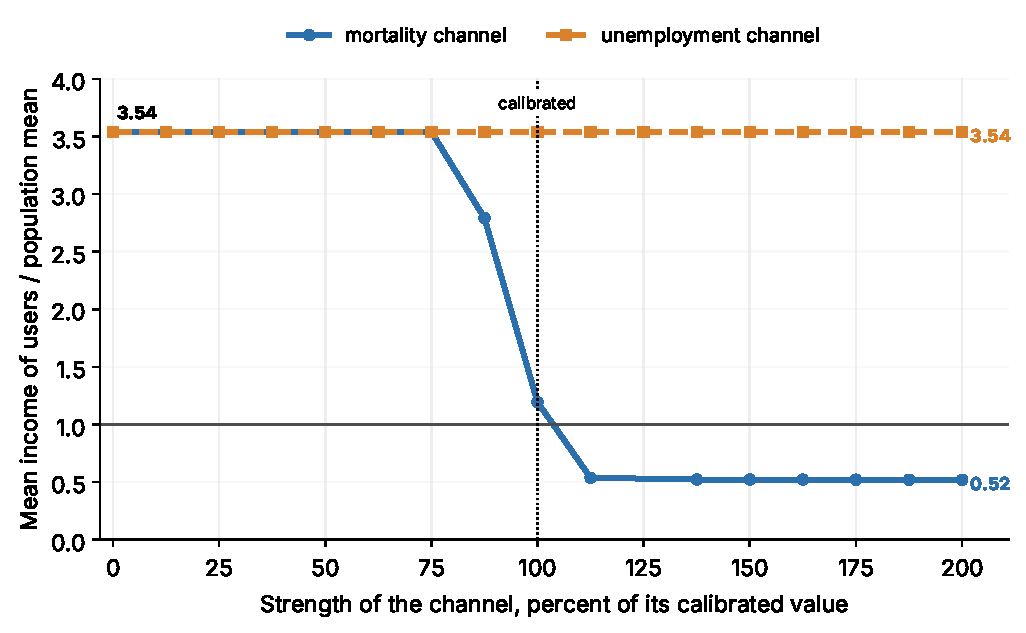
\includegraphics[width=\textwidth]{figures/stylized_who_uses.pdf}
\caption{What it takes to reverse the income gradient in drug use}
\label{fig:who}
\notes{\textwidth}{Notes: each curve scales one channel with the other switched off. Left: the model. Right: the same parameters with saving switched off. The vertical axis is average income of users over the
population average, and $b$ is recalibrated at every point so that participation is
the calibrated $8.90$ percent. The vertical dotted line marks the calibrated strength.}
\end{figure}

  Who uses depends on two things that vary with income. The first is the cost of acquiring drugs, and the second is the penalty drugs inflict. The utility cost of the drug falls with income, because a household with more income gives up less marginal utility for each dollar it spends on drugs. Therefore, ceteris paribus, drugs cost a rich household less than a poor one.

The penalty inflicted by drugs does not rise with income when it can be partially insured against, but does rise when it cannot be.   A richer household can save more to protect itself in the event of unemployment. Thus, its loss is roughly proportional to its income. As a result, in utility terms, the cost of losing its employment is about the same as the cost imposed on a poor household. Death, on the other hand, cannot be insured against.   Dying eliminates the full continuation value of being alive, and that loss grows with income, so it deters high-income households but not low-income ones. Without the ability to save, losing a job takes a household down to $\bar c$ whatever it earned, so that loss too grows with income, which is why in the right panel the unemployment channel reverses the gradient as well.

%======================================================================
\section{The quantitative model}\label{sec:full}

This section
describes the model the paper's numbers come from. It keeps the preferences of the stylized
model of Section~\ref{sec:stylized} and the two risks a SUD brings there, and adds what that model leaves out: housing, homelessness and vouchers; annual periods; unemployment insurance; income risk during working age; retirement; progressive income taxes; interest on savings; a drug-use decision in every year; recovery and treatment; SMI; a higher risk of dying, worse employment prospects and a lower chance of recovering while homeless; children who live with their parents; a drug test that misses some users; a government budget held at its benchmark net revenue; and an endogenous drug price. Notation follows
Section~\ref{sec:stylized} wherever the two models share an object: $\theta$ is the drug weight, $\sigma$ the risk aversion, $b$ the  Stone--Geary shifter, $\aleph$ the flow value of being alive, $\pi_d$ the chance that use starts a SUD, $\kappa_{\phi d}$ the mortality multiplier for the disorder, $p_v$ the drug price and $\beta$ the discount factor. The values are in Section~\ref{sec:fullcal}.

\subsection{Demographics and the state and choice sets}

At model age $j=1$, a child becomes an adult, leaves its parent's home, joins the workforce and forms its own household, with a child of its own. The household lives at most $J$ annual periods, works while $j<J_R$ and is retired from $J_R$. Its child lives with it for the first $J_K$ years and then leaves to form its own household in turn.

Each period a cohort of unit mass enters at $j=1$, made up of
the children who leave home that period, at their parent's death if that comes before $J_K$ and at $J_K$
otherwise (equation~\eqref{eq:flomnew}). It replaces the mass of the households who died, so the mass of households is constant in a stationary equilibrium. The individual state is age $j$ together with
\begin{equation}\label{eq:fstate}
s=(a,\,y,\,e,\,d,\,m,\,\eta)\in
\mathbb R_+\times\mathcal Y(j)\times\{1,2,3\}\times\{0,1,2\}\times\{0,1\}\times\{0,1,2\},
\end{equation}
where $a$ denotes assets, $y$ productivity, $e$ employment status, $d$ the SUD, $m$
SMI and $\eta$ the household's standing with the voucher programme. The SUD takes
three values because the parent's valuation of its child's prospects depends on the history of the disorder and not only on its present (Section~\ref{sec:fproblem}): $d=0$ denotes a household that has never had the disorder, $d=1$ refers to
one that had it and has recovered, and $d=2$ stands for one that has it now.\footnote{Section~\ref{sec:stylized} wrote $d\in\{0,1\}$ for the disorder absent and present; here $d=1$ is a household that has recovered, since the quantitative model keeps the history.} The
voucher state is $\eta=0$ for a household without a voucher, $\eta=1$ for one that holds one, and $\eta=2$ for one excluded from the programme after failing
Treatment First's condition (Section~\ref{sec:fvoucher}).

Each period the household chooses the bundle
\begin{equation}\label{eq:fchoice}
\big(h,\,v,\,\tau,\,a'\big)\in
\{h_1,h_2,h_3,h_4\}\times\mathbb R_+\times\{0,1\}\times\mathbb R_+ ,
\end{equation}
where $h$ is the dwelling, of which $h_1$ is a shelter, $v$ is drug consumption, $\tau$ is whether or not the household is in treatment for the SUD, available only to a household that has
the disorder, and $a'$ is its next period's assets. Labour is inelastically supplied when employed.

\subsection{Preferences}\label{sec:fprefs}

Flow utility is the stylized model's, with housing in the bundle and the child present for the first $J_K$
years. Consumption $c$ and housing $h$ are shared through the equivalence scale $\xi(j)$, which counts two members while the child is at home and one
after. The drug enters the parent's utility alone, so the parent and the child hold the bundles
\begin{equation}\label{eq:fbundles}
X_P=\Big[\Big(\frac{c}{\xi(j)}\Big)^{1-\gamma}\Big(\frac{h}{\xi(j)}\Big)^{\gamma}\Big]^{1-\theta}(b+v)^{\theta},
\qquad
X_c=\Big[\Big(\frac{c}{\xi(j)}\Big)^{1-\gamma}\Big(\frac{h}{\xi(j)}\Big)^{\gamma}\Big]^{1-\theta}b^{\theta},
\end{equation}
and period utility is
\begin{equation}\label{eq:futil}
u\big(c,h,v,\tau\big) \;=\; U(X_P)\;+\;\omega_c\,(\xi(j)-1)\,U(X_c)\;+\;\aleph\;-\;\tau\,\bar\tau^{u},
\qquad U(X)=\frac{X^{1-\sigma}}{1-\sigma}.
\end{equation}
$\gamma$ is housing's share of the non-drug bundle and $\theta$ the drug's share of
the whole, $\sigma$ is the coefficient of relative risk aversion, $\aleph$ is a flow value of being alive, counted once per household, and $\bar\tau^{u}$ is the utility
cost of a year in treatment, which is described in Section~\ref{sec:fdrug}. The child's term is its own flow utility, counted as $\xi(j)-1$ of the household and weighted by the parent at $\omega_c$. The child gets none of the drug, so a parent's drug spending reaches it through a reduction in the consumption and housing they share.

\subsection{Income, taxes and transfers}\label{sec:ftaxes}

\paragraph{Productivity.} Log productivity follows a persistent process over
working life, $\log y_{j+1}=\rho_y\log y_j+\zeta_{j+1}$ with $\zeta\sim\mathcal N(0,\sigma_\zeta^2)$, and is held fixed at its last working value in retirement.   When employed, a household earns $y\,\varepsilon(j)$. The term $\varepsilon(j)$ is a deterministic age profile, and $y$ is normalised such that it averages one upon entry. A household inherits its productivity at entry from its parent, and a child who enters with the penalty keeps a lower productivity throughout their life. I explain the intergenerational transmission in detail in Section~\ref{sec:fcosts}.

\paragraph{Before-tax income.} Before-tax income depends on age and employment,
\begin{equation}\label{eq:fincome}
\tilde y(j,y,e)=
\begin{cases}
y\,\varepsilon(j) & j<J_{R},\ e=1 \quad\text{(employed)}\\[2pt]
\psi_{ui}\,\min\{y\,\varepsilon(j),\ \bar y\} & j<J_{R},\ e=2 \quad\text{(insured, first year out of work)}\\[2pt]
0 & j<J_{R},\ e=3 \quad\text{(out of work, uninsured)}\\[2pt]
S(y) & j\ge J_{R} \quad\text{(retired)} .
\end{cases}
\end{equation}
Unemployment insurance (UI) replaces a share $\psi_{ui}$ of earnings on a base capped
at $\bar y$, and it is paid only to a share $p_{ui}$ of those losing their job, mimicking the share of
insured separations. After the first year, unemployed households, insured and uninsured alike, receive
zero UI ($e=3$). Social security $S(y)$ follows the statutory formula.\footnote{\label{fn:ss}Let $y^{s}=\min\{y,\,y^{\max}\}$ denote the household's productivity at its last
working age up to the taxable maximum $y^{\max}$, the ceiling above which earnings no longer raise the benefit. Then social security payments are $S(y)=\bar w\max\big\{\underline S,\ \alpha_1\min\{y^{s},k_1\}+\alpha_2\max\{0,\min\{y^{s},k_2\}-k_1\}
+\alpha_3\max\{0,y^{s}-k_2\}\big\}$, where $k_1<k_2$ are the two bend points,
$\alpha_1>\alpha_2>\alpha_3$ the shares replaced below, between and above them,
$\underline S$ the Supplemental Security Income (SSI) payment, and $\bar w$ the benchmark's average labour income. Their values are given in Appendix~\ref{sec:stdparams}.}

The SUD and SMI act on whether the household is employed, through the
employment transitions below. There is no
disability insurance in the model, so SMI brings no income of its own.\footnote{In the
data only a minority of adults with SMI receive disability benefits on the basis of a mental
disorder: about 3 million, through Social Security Disability Insurance or SSI, against 14.6
million adults with SMI in NSDUH 2023, roughly one in five.}

\paragraph{Taxes.} Before-tax income is taxed with the Heathcote et al.\ (2017) function
and capital income at a flat rate, so that after-tax income is
\begin{equation}\label{eq:ftax}
y^{n}=\min\big\{\tilde y,\ \tau_{\ell}\,\tilde y^{\varphi}\big\}\;+\;(1-\tau_k)\,r\,a ,
\end{equation}
where $\tau_{\ell}$ scales after-tax income and so sets the level of the tax, which falls as $\tau_{\ell}$ rises, and $1-\varphi$ sets
its progressivity. The flat tax rate on capital income is $\tau_k$, and $r$ is the exogenous interest rate on savings.\footnote{The minimum keeps the labour income tax from turning negative, since at low incomes $\tau_{\ell}\tilde y^{\varphi}$ exceeds $\tilde y$ itself.}

\paragraph{Transfers.} Food assistance pays the maximum allotment $\underline c$ less
the share $\varrho$ of income. The voucher pays a holder that is eligible this
period the part of its rent above a tenant contribution of $\kappa_r$ of income, up
to the fair market rent ($\mathit{FMR}$),
\begin{equation}\label{eq:ftrans}
\begin{aligned}
F&=\max\big\{0,\ \underline c-\varrho\,\hat y\big\},\\
V\!ch&=\mathbf{1}\{\eta=1\}\,\mathbf{1}\{\hat y<\kappa_V y^{\text{med}}\}\,\mathbf{1}\{h\neq h_1\}\,
\min\Big\{\max\{0,\ p_r h-\kappa_r\hat y\},\ \max\{0,\ \mathit{FMR}-\kappa_r\hat y\}\Big\},
\end{aligned}
\end{equation}
where $\hat y=\tilde y+ra$ is the income both programmes are means-tested on,
$\kappa_V$ and median income $y^{\text{med}}$ are the eligibility rule
in Section~\ref{sec:fvoucher}, and $\mathit{FMR}$ is the average rent paid by housed households in
the benchmark. A voucher
holder in a shelter keeps the voucher and is paid nothing until it rents again, as long as it keeps its eligibility.

Each
entering household receives a one-time endowment $T_0$ from bequests left by deceased households, and the
government collects the rest of the estates of the dead.

\subsection{The budget constraint}

The household's budget constraint is as follows:
\begin{equation}\label{eq:fbudget}
c+p_v v+a' \;=\; y^{n}+a+T_0\mathbf{1}\{j=1\}\;-\;p_r\, h\,\mathbf{1}\{h\neq h_1\}\;+\;V\!ch+F,
\qquad c\ge F,\ v\ge0,\ a'\ge0 .
\end{equation}
Food assistance is paid in kind, so it cannot directly fund the drug, the rent or saving. The
drug price is $p_v$, which is endogenous, whereas the rent per unit of housing $p_r$ is fixed and held at its benchmark value
in every simulation.\footnote{In earlier versions of this work, I solved the model with endogenous labour supply, rents, homeownership and house prices. These margins turned out to have a negligible effect on the results, so for conciseness I removed them and hold the rent fixed.} Treatment costs the household utility only; the government pays for it (see Section~\ref{sec:fgovt}).

\subsection{Housing and the homelessness loop}

Housing is the four-point grid of~\eqref{eq:fchoice}: $h_1$ is literal
homelessness, sleeping rough or in an emergency shelter, which is free, and $h_2<h_3<h_4$
are three rental sizes. Homelessness raises mortality~\eqref{eq:fsurv}, worsens both employment margins~\eqref{eq:femp} and lowers the chance of recovering from the SUD~\eqref{eq:frecover}, but does not affect SMI (Section~\ref{sec:fsmi}).

\subsection{Drug use, the SUD, recovery and treatment}\label{sec:fdrug}

A household that does not have the disorder, either $d=0$ (never had it) or $d=1$ (had it
but recovered), acquires it ($d=2$) with probability $\pi_d$ if it uses,\footnote{In earlier versions of the model, I allowed the probability of developing a SUD to rise with use, but since it had little impact on the results, I removed it for simplicity.}
\begin{equation}\label{eq:fd}
\Pr(d'=2\mid d\neq 2,\,v)=\pi_d\,\mathbf{1}\{v>0\},
\end{equation}
and a household that has
recovered can acquire the disorder again. A household may begin using only up to an
age $J_E$.\footnote{\label{fn:je}Without this limit, using at old ages has little-to-no consequence: too
little life remains for the disorder to damage, so the model produces too much old-age use. The cause is that death is certain at the last age $J$, so close to it a household
knows how little life remains, whereas in real life the vast majority of people do not know exactly when they will die.
 The value of $J_E$ is in Appendix~\ref{sec:stdparams}.  The limit stops only households without a SUD from starting to use; a household that already has a SUD at that age keeps using.} A household with the SUD recovers, to $d=1$, with probability
\begin{equation}\label{eq:frecover}
\begin{aligned}
\pi_r(h,m,\tau)=\min\Big\{1,\ \bar\pi_r\,&\big(\mathbf{1}\{h=h_1\}\,\mu_H+\mathbf{1}\{h\neq h_1\}\big)\big(\mathbf{1}\{m=1\}\,\mu_m+\mathbf{1}\{m=0\}\big)\\
&\times\big(\mathbf{1}\{\tau=1\}\,g+\mathbf{1}\{\tau=0\}\big)\Big\},
\end{aligned}
\end{equation}
where $\bar\pi_r$ is the baseline annual chance of recovering while housed, without SMI and untreated.   Three multipliers affect it. Recovery is harder when homeless ($\mu_H<1$) as well as with SMI ($\mu_m<1$), but is more likely in treatment ($g>1$).

 Households who go to treatment $\tau$ pay a utility cost $\bar\tau^u$, shown in~\eqref{eq:futil}. What they gain is a higher chance of recovery, with $g>1$. Treatment does not require a household to stop using, but as long as the disorder remains, it still raises the risk of mortality.

\subsection{SMI}\label{sec:fsmi}

$m$ is a two-state Markov chain representing SMI, mental illness severe enough to cause substantial functional impairment. It affects a small share of adults, whereas any
mental illness affects roughly a quarter of adults and includes mild anxiety. Onset
follows an age profile $\varsigma_m(j)$, normalised to one at age $26$ and scaled by the level
$\omega_m$, and a household that carries the SUD is $\iota>1$ times more likely to develop SMI than one that does not,
\begin{equation}\label{eq:fonset}
\Pr(m'=1\mid m=0,d)=\min\big\{1,\ \omega_m\,\varsigma_m(j)\,\big(\mathbf{1}\{d=2\}\,\iota+\mathbf{1}\{d\neq2\}\big)\big\},
\qquad
\Pr(m'=0\mid m=1)=\lambda_m .
\end{equation}
A household with SMI recovers from it with the probability $\lambda_m$ each year, whatever its housing and whether or not it carries the SUD.

SMI then affects three objects: the chance of finding a job when unemployed, through~\eqref{eq:femp}; mortality, through~\eqref{eq:fsurv}, both in
Section~\ref{sec:fcosts}; and the SUD recovery hazard, through $\mu_m$
in~\eqref{eq:frecover} in Section~\ref{sec:fdrug}. It does not enter the utility function.

The SMI chain does not depend on housing, because in the At Home / Chez Soi randomised trial, housing had no detectable effect on the symptoms of homeless adults with SMI (Stergiopoulos et al., 2015).

\subsection{What the SUD, SMI, and homelessness cost}\label{sec:fcosts}

\paragraph{Death risk.}\label{sec:fdeath} Write $1-\bar\phi(j)$ for the probability of dying
at age $j$ of a household that is housed and has neither the disorder nor SMI; the three
multipliers below raise it for every other household. Write
$q^{\,0}(j,h)=\min\{1,\big(\mathbf{1}\{h=h_1\}\,\kappa_{\phi H}+\mathbf{1}\{h\neq h_1\}\big)\,(1-\bar\phi(j))\}$ and
$q^{\,1}(j,h)=\min\{1,\kappa_{\phi d}\,\big(\mathbf{1}\{h=h_1\}\,\kappa_{\phi H}+\mathbf{1}\{h\neq h_1\}\big)\,(1-\bar\phi(j))\}$
for the probability of dying without and with the disorder, respectively. In the stylized model $\kappa_{\phi d}$ was an exponent on the survival probability; here it multiplies the death hazard. The probability of dying is then
\begin{equation}\label{eq:fsurv}
1-\phi(j,h,d,m)=\min\Big\{1,\ \big(\mathbf{1}\{m=1\}\,\kappa_{\phi m}+\mathbf{1}\{m=0\}\big)\,q^{\,0}(j,h)
+\mathbf{1}\{d=2\}\big[q^{\,1}(j,h)-q^{\,0}(j,h)\big]\Big\},
\end{equation}
so $\kappa_{\phi H}{}>1$ multiplies the death probability when a household is in a shelter, $\kappa_{\phi d}{}>1$ when a household has a SUD, and $\kappa_{\phi m}>1$ the baseline risk when a household has SMI, to which the excess risk of the disorder is
added.

\paragraph{Unemployment risk.} A job is lost with probability $\pi^{eu}$ and found
with probability $\pi^{ue}$,
\begin{equation}\label{eq:femp}
\begin{aligned}
\pi^{eu}(y,h)&=\min\Big\{1,\ \bar\pi^{eu}\,\varpi(y)\,
\big(1+\mathbf{1}\{h=h_1\}\,\kappa_{H}\big)\Big\},\\
\pi^{ue}(h,d',m')&=\min\Big\{1,\ \frac{\bar\pi^{ue}\,\big(1-\mathbf{1}\{h=h_1\}\,\kappa_{H}\big)}
{\big(\mathbf{1}\{d'=2\}\,\kappa^{ue}_{d}+\mathbf{1}\{d'\neq2\}\big)\big(\mathbf{1}\{m'=1\}\,\kappa^{ue}_{m}+\mathbf{1}\{m'=0\}\big)}\Big\},
\end{aligned}
\end{equation}
with $\bar\pi^{eu}$ and $\bar\pi^{ue}$ the baseline separation and job-finding rates,
$\varpi(y)$ a factor that makes separations likelier at low productivity, and the divisors
$\kappa^{ue}_{d}$ and $\kappa^{ue}_{m}$ making a job harder to find with the SUD and with
SMI. Neither the SUD nor SMI raises separations; each only reduces the chance of regaining employment. $\kappa_{H}$ does both for a household in a
shelter.

\paragraph{The child's productivity penalty.} A child whose parent had the disorder at any point while the child lived at home,
before $J_K$ or before the parent died if that came first, starts adult life with its productivity lowered
by the proportion $\delta_d$ in~\eqref{eq:fnewborn} below, and the penalty stays with the
child for life.

A child's log productivity at entry is drawn around its parent's, with persistence $\rho$. The innovation keeps the spread of productivity at entry the same in every generation. If the parent had the disorder at any point before the child became an adult, the penalty scales the child's productivity down for life:

\begin{equation}\label{eq:fnewborn}
\begin{aligned}
\log y_{1}^{\text{child}}\;=\;&\rho\,\log y^{\text{parent}}+(1-\rho)\,\mu+\epsilon\\
&+\log(1-\delta_d)\,\mathbf{1}\{\text{parent has } d\ge1 \text{ when its child becomes an adult}\},
\end{aligned}
\end{equation}
with $y_1^{\text{child}}$ the child's productivity in the period it becomes an adult in the workforce ($j=1$), $y^{\text{parent}}$ the parent's productivity in the period just before its child becomes an adult, $\mu$
the mean of log productivity at entry and $\epsilon$ normally distributed with mean zero and
variance $1-\rho^2$ times the variance of log productivity at entry.   The penalised child's productivity is lower, which means that its own child is also more likely to inherit a lower draw. Through this persistence, the penalty ripples through the whole lineage, and not just the child whose parent had a SUD during their childhood.

\subsection{The voucher and the two policies}\label{sec:fvoucher}

A household is eligible for a voucher while its income is below the share
$\kappa_V$ of median income,
\begin{equation}\label{eq:felig}
\hat y\;<\;\kappa_V\,y^{\text{med}},
\end{equation}
with $\hat y$ the income of~\eqref{eq:ftrans}. A holder keeps its voucher while it is
eligible, and an eligible household without one draws one with probability
$\pi_V$. Under Housing First that is the whole rule.

Under Treatment First the programme is conditional. A household fails the condition if
it uses, $v>0$, or has the disorder and is not in treatment, $d=2$ and $\tau=0$. A household with a SUD must be in treatment (paid for by the government), as the executive order directs, and no household may use even while in treatment, as the guidance implementing the order requires of drug-free housing.\footnote{ Executive Order 14321, Section 5(b); the guidance is \emph{Addressing Homelessness and Addiction through ``Treatment First''} (2026), p.~9, issued by the Office of National Drug Control Policy, the Department of Health and Human Services and HUD. The Housing Choice Voucher programme bars admission for current illegal drug use (Code of Federal Regulations (CFR), Title 24, Section 982.553) but does not test; Housing First here is a programme that does not test. The order also encourages the civil commitment of people with mental illness who pose a risk to themselves or others, or who live on the street and cannot care for themselves. In the model, treatment is always the household's choice: a household with a SUD that declines it loses its voucher if the screen catches it.}

Income-eligible holders and income-eligible households that draw a voucher are tested, at a cost
$c_{\text{test}}$ each to the government, and one that fails the condition is detected with probability
$p_{\text{det}}$. This means that enforcement is not perfect: with probability $1-p_{\text{det}}>0$ a household that fails the condition actually gets to keep its voucher. A detected holder keeps this period's payment
and loses the voucher from the next period; a detected applicant never receives it. In both cases,
the household is excluded from the voucher programme for a period of time ($\eta=2$): it cannot draw a voucher whatever its income, and it
returns to the lottery ($\eta=0$) with probability $\psi_x$ each year.

None of
$p_{\text{det}}$, $\psi_x$ and $c_{\text{test}}$ binds in the benchmark, where no voucher
is conditional, so all three are set with the experiment in
Section~\ref{sec:experiments} rather than in the calibration.

\subsection{The household's dynamic problem}\label{sec:fproblem}

Write $\Gamma\big(s'\mid s,\,h,v,\tau,a'\big)$ for the law of motion of the state that the transitions above define, given the state and the choices. Then, for $j=1,\dots,J$ and with $V(J{+}1,\cdot)=0$,
\begin{equation}\label{eq:fbellman}
\begin{aligned}
V(j,s)=\max_{\{h,\,v,\,\tau,\,a'\}}\ \Bigg\{\
&U(X_P)+\omega_c(\xi(j)-1)\,U(X_c)+\aleph-\tau\bar\tau^{u}\\[2pt]
&+\ \beta\,\phi(j,h,d,m)\!\int_{\mathcal S}\! V(j{+}1,s')\,
\Gamma\big(\mathrm{d}s'\mid s,h,v,\tau,a'\big)\\[2pt]
&-\ \beta\,\chi(j)\,\omega_c\,D(y,d)\Bigg\},
\qquad
\chi(j)=\begin{cases}1-\phi(j,h,d,m) & j<J_K\\ 1 & j=J_K\\ 0 & j>J_K,\end{cases}
\end{aligned}
\end{equation}
subject to the budget~\eqref{eq:fbudget}, the income and transfer
rules~\eqref{eq:fincome} to~\eqref{eq:ftrans} in Section~\ref{sec:ftaxes}, and the restrictions that treatment is
available only to a household with $d=2$ and that no household begins using after $J_E$.

The first line is the flow of~\eqref{eq:futil}. The second is the household's own
continuation. The third is the impact of the parent on the child's adult value, counted only when the child leaves: at
$J_K$ with certainty, and before then with the probability that the parent dies first.
$D(y,d)$ is what the parent's disorder costs the child, in the child's own lifetime value,
\begin{equation}\label{eq:fchild}
D(y,d)=\mathbb{E}\big[V(1,s_{\text{child}})\,\big|\,y,\ 0\big]
-\mathbb{E}\big[V(1,s_{\text{child}})\,\big|\,y,\ d\big]\;\ge\;0,
\end{equation}
where the child is valued as it enters at $j=1$ with the initial states described in Section~\ref{sec:fnewbornsec}, and its productivity is drawn as
in~\eqref{eq:fnewborn} in Section~\ref{sec:fcosts} from a parent with productivity $y$. In the first term of~\eqref{eq:fchild} the parent has never had the disorder, and in the second it has its actual $d$ in the period the child leaves. If it never had a SUD, there is no charge to the parent ($D(y,0)=0$); if it had a SUD before the child leaves ($d\ge1$), it is charged ($D(y,d)>0$).\footnote{The term is a difference and not a level. Written as a level, $\omega_c$ times the child's value, the term would be worth more to a household the likelier the household is to die, because the death branch carries it. It would then pay most to the households with a SUD, for reasons that have nothing to do with the child. As a difference, the term is zero for a parent who has never had the disorder and a cost otherwise.}

One weight $\omega_c$ multiplies both child terms, the flow of childhood and the value
of the child's adulthood. At $\omega_c=0$ the damage a household does to its child is entirely
external; at $\omega_c>0$ it internalises the share $\omega_c$ and only $1-\omega_c$
remains external.

The policy functions $h(j,s)$, $v(j,s)$, $\tau(j,s)$ and $a'(j,s)$ are the dwelling, drug use, treatment and saving that solve~\eqref{eq:fbellman} at age $j$ and state $s$.

\subsection{The government}\label{sec:fgovt}

Write $\Phi(j,s)$ for the distribution of the households of age $j$ over the states $s$; its law of motion is in Section~\ref{sec:fnewbornsec}. The government's budget constraint is
\begin{equation}\label{eq:fgovt}
\begin{aligned}
\mathcal R\;=\;&\sum_{j=1}^{J}\int_{\mathcal S}\Big[\,\tilde y(j,y,e)-\min\big\{\tilde y(j,y,e),\,\tau_{\ell}\,\tilde y(j,y,e)^{\varphi}\big\}+\tau_k\,r\,a\\
&\qquad\quad+\big(1-\phi\big(j,h(j,s),d,m\big)\big)\,a'(j,s)\,\Big]\,\mathrm d\Phi(j,s)\;-\;T_0\\
&-\sum_{j=1}^{J}\int_{\mathcal S}\Big[\,U\!I(j,y,e)+S(j,y)+F(j,s)+V\!ch(j,s)+c_{\text{test}}\,\mathbf{1}^{\text{test}}(j,s)+c_{\text{treat}}\,\mathbf 1\{d=2,\,\tau(j,s)=1\}\,\Big]\,\mathrm d\Phi(j,s).
\end{aligned}
\end{equation}
The first line is revenue from the labour and capital income taxes of~\eqref{eq:ftax}. The second is the estates of the households who die, which the government collects, less the endowment $T_0$ it gives the unit mass of entrants. The third is what the government pays: UI, $U\!I(j,y,e)=\tilde y(j,y,e)\,\mathbf 1\{j<J_R,\,e=2\}$; social security, $S(j,y)=S(y)\,\mathbf 1\{j\ge J_R\}$; food assistance $F(j,s)$ and the voucher $V\!ch(j,s)$ of~\eqref{eq:ftrans}, at the household's dwelling $h(j,s)$; under Treatment First, the cost $c_{\text{test}}$ of each household tested, $\mathbf{1}^{\text{test}}(j,s)=1$; and, under both policies, the cost $c_{\text{treat}}$ of a year of treatment for each household with the SUD that takes it up, $\tau(j,s)=1$, since treatment is publicly funded.

In the benchmark the tax parameters are set as in Section~\ref{sec:fullcal} and
$\mathcal R$ is whatever surplus they produce. In every experiment the taxes are
held at their benchmark values, and the probability of drawing a voucher $\pi_V$ adjusts
so that $\mathcal R$ equals its benchmark value $\bar{\mathcal R}$, unless the experiment fixes $\pi_V$.

\subsection{The drug market}

The price of the drug clears its market,
\begin{equation}\label{eq:fdrug}
p_v=\nu_1 S_v^{1/\varepsilon_s},
\qquad S_v=\sum_{j=1}^{J}\int v(j,s)\,\mathrm{d}\Phi(j,s),
\end{equation}
where $\varepsilon_s$ is the price elasticity of supply and $\nu_1$ is normalised so
that the price is one in the benchmark, and then held fixed across experiments.\footnote{The suppliers are outside the economy: what they earn along the supply curve is counted neither in welfare nor in the budget.}

\subsection{The law of motion}\label{sec:fnewbornsec}

Given the policy functions, the distribution over states evolves by pushing
households through their choices and then through the shocks,
\begin{equation}\label{eq:flom}
\Phi(j{+}1,\mathcal S')\;=\;\int_{\mathcal S}\!\phi\big(j,h(j,s),d,m\big)\,
\Gamma\big(\mathcal S'\mid s,\,h(j,s),v(j,s),\tau(j,s),a'(j,s)\big)\,
\mathrm{d}\Phi(j,s),
\end{equation}
for $j=1,\dots,J-1$ and every measurable set $\mathcal S'$ of the state space $\mathcal S$ of~\eqref{eq:fstate}, with the integral over the state $s$ of the households of age $j$, together with the inflow of entrants
\begin{equation}\label{eq:flomnew}
\Phi(1,\mathcal S')\;=\;\frac{\sum_{j\le J_K}\int_{\mathcal S}\!\chi(j)\,
\mathcal N\big(\mathcal S'\mid s\big)\,\mathrm{d}\Phi(j,s)}
{\sum_{j\le J_K}\int_{\mathcal S}\!\chi(j)\,\mathrm{d}\Phi(j,s)},
\end{equation}
where the integrals are again over $s$, $\mathcal N$ places the child according
to~\eqref{eq:fnewborn} and $\chi(j)$ is the weight defined in Section~\ref{sec:fproblem}. An entrant starts with the endowment $T_0$, is employed, has never had the disorder, holds no voucher, and carries SMI with the prevalence observed at age 26.\footnote{A disorder acquired before that age is therefore acquired in the model only after entry; however, the share of adults with a SUD still matches the data (Section~\ref{sec:fullcal}).}

\subsection{Competitive equilibrium}

A competitive equilibrium is a collection of
\begin{itemize}\setlength{\itemsep}{0em}\setlength{\parskip}{0em}
\item value functions $\big\{\{V_t(j,\cdot)\}_{j=1}^{J}\big\}_{t=0}^{\infty}$;
\item policy functions
$\big\{\{h_t(j,\cdot),\,v_t(j,\cdot),\,\tau_t(j,\cdot),\,a'_t(j,\cdot)\}_{j=1}^{J}\big\}_{t=0}^{\infty}$;
\item distributions $\big\{\{\Phi_t(j,\cdot)\}_{j=1}^{J}\big\}_{t=0}^{\infty}$; and
\item prices, policies and aggregates
$\big\{p_{vt},\,\pi_{Vt}\big\}_{t=0}^{\infty}$, together with $\bar y$, $y^{\text{med}}$ and
$\mathit{FMR}$, which carry no date because they are kept fixed at their benchmark values,
\end{itemize}
such that, at every date $t$,
\begin{enumerate}\setlength{\itemsep}{0.1em}\setlength{\parskip}{0em}
\item the policy functions solve~\eqref{eq:fbellman} given its terminal condition, and
$\{V_t(j,\cdot)\}_{j=1}^{J}$ are the associated values;
\item $\Phi_{t+1}(j{+}1,\cdot)$ follows from $\Phi_t(j,\cdot)$ by the law of
motion~\eqref{eq:flom} together with the entrants of~\eqref{eq:flomnew}
and~\eqref{eq:fnewborn};
\item the government budget~\eqref{eq:fgovt} holds at
$\pi_{Vt}$ with $\mathcal R=\bar{\mathcal R}$;
\item the drug market clears at $p_{vt}$, so~\eqref{eq:fdrug} holds.
\end{enumerate}
  A stationary equilibrium is a special case in which all objects are constant. I calibrate the model in a stationary equilibrium, and the long-run policy comparisons also report stationary equilibria. When I hold $\pi_V$ or the drug price at their benchmark values in any experiment, I exclude the budget condition or the drug-market condition, respectively.

\section{Calibrating the quantitative model}\label{sec:fullcal}

The model has fifty-nine parameters, some of which vary by age. Thirty-eight are calibrated externally, from data or the literature, and twenty-one internally. The twenty-six that carry this paper's story are in Table~\ref{tab:eleven}, with the moment, source, data and model value behind each, and are discussed below in numbered blocks of parameters that work through similar mechanisms. The other thirty-three, common to most life-cycle models, are in Appendix~\ref{sec:stdparams} to save the reader time; its blocks continue the numbering. Three further parameters govern drug testing and exclusion from the voucher; they play no role in the benchmark and are set with the experiment in Section~\ref{sec:experiments}. \texttt{data/DATA\_APPENDIX.md} in the replication package documents the dataset, year, universe and computation behind every estimate, and the package carries all datasets, so nothing has to be downloaded.

\subsection{The twenty-six parameters that carry the story of this paper}\label{sec:fmainpar}

\begin{table}[htbp]\centering
\caption{\normalsize The twenty seven parameters that carry the story of this paper}\label{tab:eleven}
\begingroup\scriptsize\setlength{\tabcolsep}{2pt}
\begin{tabular}{@{}lL{123pt}cL{238pt}r@{}}
\toprule
Parameter & Description & Set & Moment and source & Value \\
\midrule
\multicolumn{5}{@{}l}{\emph{Who uses drugs}} \\
$b$ & Whether a household uses & Int. & Drug participation, NSDUH 2024 & \textemdash \\
$\lambda$ & SUD hazard per unit used & Int. & Users acquiring a SUD, NSDUH 2024 & \textemdash \\
$\bar\kappa_{\phi d}$ & Mortality with a SUD & Ext. & Mortality ratios, Hjorth\o j et al.\ (2023) & 8.00 \\
$\aleph$ & Flow value of being alive & Int. & Value of a statistical life, Viscusi (2003) & \textemdash \\
\addlinespace
\multicolumn{5}{@{}l}{\emph{\textcolor{red}{What using and being homeless cost}}} \\
$\rho_d$ & Earnings lost to a SUD & Int. & Employment rate of the homeless, HUD 2023 & \textemdash \\
$\kappa_{ued}$ & Employment multiplier, SUD & Int. & Unemployment rate given a SUD, NSDUH 2024 & \textemdash \\
$h_1$ & Service flow of homelessness & Int. & Homelessness rate, HUD 2023 & \textemdash \\
$\kappa_{\phi H}(j)$ & Increased mortality when homeless & Ext. & Mortality ratios by age, Baggett et al.\ (2013) & 4.41 to 1.09 \\
$\kappa_{ueH}$ & Employment multiplier, homeless & Ext. & Desmond and Gershenson (2016) & 0.80 \\
\textcolor{red}{$\zeta_{DI}$} & \textcolor{red}{Disability replacement, SMI} & \textcolor{red}{Ext.} & \textcolor{red}{SSDI and SSI rates, SSA 2023} & \textcolor{red}{0.25} \\
$\pi_V$ & Voucher lottery probability & Int. & Recipients over eligible, HUD 2023 & \textemdash \\
\addlinespace
\multicolumn{5}{@{}l}{\emph{\textcolor{red}{The mental illness chain}}} \\
\textcolor{red}{$p_m$} & \textcolor{red}{Prevalence the onset reproduces} & \textcolor{red}{Ext.} & \textcolor{red}{Share with SMI, NSDUH 2023} & \textcolor{red}{5.5\%} \\
\textcolor{red}{$\lambda_m$} & \textcolor{red}{Annual chance of leaving SMI} & \textcolor{red}{Int.} & \textcolor{red}{SMI share of homeless, Gutwinski et al.\ (2021)} & \textcolor{red}{\textemdash} \\
\textcolor{red}{$\iota$} & \textcolor{red}{SUD multiplier on SMI onset} & \textcolor{red}{Ext.} & \textcolor{red}{Danish registers, Nielsen et al.\ (2017)} & \textcolor{red}{2.00} \\
$\rho_m$ & Earnings lost to SMI & Int. & Earnings of workers with SMI, NSDUH 2023 & \textemdash \\
$\kappa_{uem}$ & Employment multiplier, SMI & Int. & Employment rate given SMI, NSDUH 2023 & \textemdash \\
\textcolor{red}{$\mu_m$} & \textcolor{red}{SUD recovery multiplier, SMI} & \textcolor{red}{Ext.} & \textcolor{red}{Dual diagnosis relapse, Bradizza et al.\ (2006)} & \textcolor{red}{0.82} \\
\textcolor{red}{$\kappa_{\phi m}$} & \textcolor{red}{Mortality multiplier, SMI} & \textcolor{red}{Ext.} & \textcolor{red}{Olfson et al.\ (2015)} & \textcolor{red}{2.50} \\
\addlinespace
\multicolumn{5}{@{}l}{\emph{\textcolor{red}{Recovery and treatment}}} \\
\textcolor{red}{$\bar\pi_r$} & \textcolor{red}{Baseline SUD recovery rate} & \textcolor{red}{Ext.} & \textcolor{red}{Ten year remission rate, Vaillant (1995)} & \textcolor{red}{0.025} \\
$\mu_H$ & Recovery multiplier when homeless & Int. & Weeks abstinent, Milby et al.\ (2005) & \textemdash \\
\textcolor{red}{$g$} & \textcolor{red}{Treatment effect on recovery} & \textcolor{red}{Ext.} & \textcolor{red}{Odds ratio, Milby et al.\ (2005)} & \textcolor{red}{1.35} \\
\textcolor{red}{$\bar\tau^{u}$} & \textcolor{red}{Utility cost of treatment} & \textcolor{red}{Int.} & \textcolor{red}{Treatment take up, NSDUH 2023} & \textcolor{red}{\textemdash} \\
\addlinespace
\multicolumn{5}{@{}l}{\emph{The externalities}} \\
$\omega$ & Weight on the child & Int. & Parent use rate with a child, NSDUH 2024 & \textemdash \\
$\delta_d$ & Child's earnings, parent SUD & Int. & Child SUD ratio, McGovern et al.\ (2023) & \textemdash \\
$\delta_h$ & Child's earnings, homeless & Ext. & Poverty exposure on child's earnings, Chetty et al.\ (2016) & 0.31 \\
$\omega_{\ell}$ & Weight on leisure & Int. & Average hours worked, Guvenen et al.\ (2023) & \textemdash \\
$\kappa_x$ & Disamenity of homelessness & Ext. & Willingness to pay to eliminate homelessness, Loubi\`ere et al.\ (2020) & 0.0008 \\
\bottomrule
\end{tabular}
\endgroup
\end{table}


\paragraph{Block 1: Who uses drugs.}  The five parameters in this block decide the share of participants and who participates.  They decide how much there is for a policy to affect.
\begin{description}\setlength{\itemsep}{0.25em}\setlength{\parskip}{0em}
\item[$\theta$, the weight on drugs in utility.]
  The weight in utility given to drugs mostly determines what share of its budget a household that uses drugs spends on drugs. To a lesser extent, a higher weight also makes using at all more attractive. As it rises, use therefore rises on both the extensive and the intensive margin, and with it the externalities and what either policy has to act on. It is calibrated internally, at $0.17$, to aggregate drug spending by users over their aggregate income, $16.0$ percent, from retail drug spending in Midgette et al.\ (2019) and, in NSDUH 2024, the incomes of adults aged 26 and over who use drugs.

\item[$b$, the marginal utility from the first unit of drugs.] The marginal value of the first unit of drugs goes as $\theta/b$, so a larger $b$ makes the first units worth less and a household with little to spend buys none. As $b$ falls, the marginal utility from the first unit rises, and so do overall drug use and the externalities that policy can affect. It targets a participation rate of $8.90$ percent, the NSDUH 2024 rate of a drug use disorder of any severity among adults aged 26 and over.\footnote{A user in the model is therefore a household whose use of any illicit drug, marijuana among them, amounts to a disorder, mild included. A household with a SUD is one whose disorder is moderate or severe (next item). Use that never reaches a disorder is not modelled.}
\item[$\pi_d$, the chance that a year of use leads to a SUD.]   By governing how likely drug use is to become a disorder, this parameter determines how risky drug use is. When it rises, the externalities and moral hazard grow. It targets the share of users who have a SUD, $41.3$ percent among adults aged 26 and over in NSDUH 2024.
\item[$\kappa_{\phi d}$, increased mortality with a SUD.] $\kappa_{\phi d}$ sets how much a SUD raises the chance of dying, and mortality truncates a user's value of life. Because this is an uninsurable risk, a rise in $\kappa_{\phi d}$ hits the households with the highest values of life hardest, which reverses the income gradient; as the stylized model of Section~\ref{sec:stylized} shows, this makes it a key parameter. It is calibrated internally, at $4.00$, to the income of users relative to the average, a value within the range of the mortality rate ratios of a SUD in the literature: $3.91$ in the Danish registers (Plana-Ripoll et al., 2019) and $6.6$ among Norwegians in specialist care for a SUD (Heiberg et al., 2018). Users earn $62$ percent of the average in the model against $74$ percent in the data.
\item[$\aleph$, the flow value of being alive.]   While $\kappa_{\phi d}$ sets how much a SUD raises the chance of dying, $\aleph$ decides the value of life. As it rises, dying costs more and use falls. It targets a VSL of $80$ times average labour income (Viscusi and Aldy, 2003).\footnote{No household has a negative value of life in equilibrium, so death is never optimal. Because the value of being alive enters utility additively and utility is concave, the VSL rises faster than consumption, roughly with its square at the model's risk aversion, as in Hall and Jones (2007). Estimates of the income elasticity of the VSL are lower across people at a point in time, $0.5$ to $0.6$ in Viscusi and Aldy (2003), than over time, $1.5$ to $1.7$ in Costa and Kahn (2004).}
\end{description}

\paragraph{Block 2: Costs of homelessness and vouchers.} Both policies work on this block, from opposite ends: each parameter says how welfare reducing a state is, and so what a voucher and its removal are worth in it.
\begin{description}\setlength{\itemsep}{0.25em}\setlength{\parskip}{0em}
\item[$\kappa^{ue}_{d}$, how much less likely it is to regain employment with a SUD.] An unemployed household with a SUD finds work at the rate $\bar\pi^{ue}$ divided by $\kappa^{ue}_{d}{}>1$. As $\kappa^{ue}_{d}$ rises, the expected unemployment spells of households with a SUD lengthen and they are likelier to lose their housing: this is the link from the disorder to the street, and it shapes how much Treatment First deters. It is calibrated internally to the SUD share of the homeless, $21.7$ percent in Gutwinski et al.\ (2021).
\item[$h_1$, the service flow of homelessness.] This parameter sets how welfare reducing the outside option is, which affects the value of life: a household with little to lose from dying faces a smaller mortality cost of using. As $h_1$ rises, a shelter is less welfare reducing, a voucher is worth less and Treatment First has less to act on. It targets a homelessness rate within 0.40 to 1.00 percent of households: the floor is HUD's 2023 PiT count, which counts a single night; the ceiling is the share homeless at some point over a year, from Burt et al.\ (2001). Its value is $53$ percent of the smallest rental (Appendix~\ref{sec:stdparams}), and the model delivers an aggregate homelessness rate of $0.62$ percent.
\item[$\kappa_{\phi H}$, mortality when homeless.] This parameter sets how much more likely a homeless household is to die. As it rises, the cost of homelessness rises, a voucher is worth more and Treatment First's deterrence is stronger. It is set externally to multiply baseline mortality by $1.60$ at every age, the mortality ratio for homeless adults against poor housed adults in Meyer et al.\ (2023).
\item[$\kappa_{H}$, the employment penalty of homelessness.] This parameter sets how much likelier a household in a shelter is to lose its job and how much less likely it is to find one: separations are $1+\kappa_H$ times as frequent and job finding $1-\kappa_H$ times as fast. Housing First recovers that employment directly, whereas Treatment First does so only as the fall in SUD lowers unemployment and homelessness over time. As $\kappa_H$ rises, homelessness costs more, and both policies have more to act on. It is set externally at $0.20$, from Desmond and Gershenson (2016).
\item[$\underline c$, the food stamp maximum allotment.] This parameter sets how low consumption can go for the poorest households, with no income, assets or voucher, and so where utility is bounded from below. As it rises, the value of being alive rises, mortality costs more and Treatment First has more to deter. It is calibrated internally to food stamp spending over output, $0.42$ percent: outlays from the United States Department of Agriculture (USDA) over GDP.
\item[$\pi_V$, the chance of drawing a voucher.] This is the policy dial itself, and it holds the whole trade-off. Raising it houses more households, which reduces the \emph{childhood homelessness externality}, and makes life worth more, which makes Treatment First's deterrence more effective. In the benchmark it is calibrated internally, at $0.068$, so that the share of income-eligible households who hold a voucher is aligned with the $26.6$ percent in HUD's Picture of Subsidized Households, 2023.
\item[$T_0$, the endowment at entry to adulthood ($j=1$).] A child who becomes an adult starts adult life with $T_0$ times average earnings, which sets how likely a young adult is to end up in a shelter in its first years.   As it rises, fewer parents are homeless, and Treatment First has less of an effect on drug use during parenthood, and thus less of an effect on children. Its moment is the share of the homeless aged 25 to 34, $26.0$ percent in HUD's 2024 PiT count.
\end{description}

\paragraph{Block 3: SMI chain.}   This block determines how much  Treatment First prevents beyond drug use and SUD. This is because a SUD raises the chance of SMI, and SMI lowers employment and raises mortality.
\begin{description}\setlength{\itemsep}{0.25em}\setlength{\parskip}{0em}
\item[$\iota$, the SUD multiplier on SMI onset.]   This is the key parameter of this block because it determines how much a SUD affects the onset of SMI. As it rises, a SUD increases the prevalence of SMI more, and Treatment First reaches further, because preventing the disorder then also lowers overall SMI. It is set externally at $2.00$, between the hazard ratio of $1.34$ for any SUD that Hjorth\o j et al.\ (2018) estimate for the conversion from schizotypal disorder to schizophrenia and the $6.04$ for any substance abuse that Nielsen et al.\ (2017) estimate for the onset of schizophrenia, both in the Danish registers.
\item[$\lambda_m$, the annual chance of recovering from SMI.]   This parameter determines how long an SMI spell is expected to last. As it rises, SMI becomes less persistent and Treatment First's deterrence of drug use declines, because the SMI spells a SUD can trigger are shorter on average. I set it externally to $0.066$, which is an annual hazard consistent with the ten-year recovery rate of $50$ percent for bipolar disorder in {\AA}sb{\o} et al.\ (2022).
\item[$\omega_m$, the level of the SMI onset profile.]   This parameter scales the probability of developing SMI at every age. As it rises, a SUD has a larger effect on SMI, and Treatment First reaches further than just drug use and SUD. It is calibrated internally to the share of the population with SMI, $4.82$ percent, the prevalence in NSDUH 2024.
\item[$\kappa^{ue}_{m}$, how much less likely it is to regain employment with SMI.] The same as $\kappa^{ue}_{d}$ for SMI: a household with SMI finds work at the rate $\bar\pi^{ue}$ divided by $\kappa^{ue}_{m}{}>1$. As it rises, expected unemployment spells with SMI lengthen and SMI costs more. Its moment is the SMI share of the homeless, $25$ percent in Gutwinski et al.\ (2021), since a household out of work longer is likelier to become homeless.
\item[$\mu_m$, the SUD recovery multiplier for SMI.] The chain's second direction: a SUD raises the chance of SMI, and SMI makes a SUD more persistent. As it falls, recovering from a SUD is less likely, and Treatment First has more to overcome. It is set externally at $0.82$ from the dual-diagnosis relapse rates in Bradizza et al.\ (2006).
\item[$\kappa_{\phi m}$, the mortality multiplier for SMI.] The chain's last link, through which SMI shortens life. As it rises, more households with SMI die, and Treatment First has more to work on, because less drug use means less SUD, less SMI and fewer deaths. It is set externally at $2.50$, the middle of the standardised mortality ratios for SMI in Olfson et al.\ (2015).
\end{description}

\paragraph{Block 4: Recovery and treatment.} Both policies work through this block: Treatment First encourages seeking treatment, and Housing First buys recovery by housing people, since recovery is likelier while housed.  The first two parameters determine how quickly recovery happens, the next two decide how much treatment raises recovery and how likely a household with a SUD is to go to treatment, and the last parameter determines how much it costs the government to send a household to treatment for a SUD.
\begin{description}\setlength{\itemsep}{0.25em}\setlength{\parskip}{0em}
\item[$\bar\pi_r$, the baseline SUD recovery rate.] This parameter is the annual chance that a housed household recovers from a SUD, the level everything else in the block scales. As it rises, disorders are expected to end more quickly on their own, and there is less for either policy to do. It is set externally at $0.025$, the annual hazard implied by the ten-year remission rate in Vaillant (1995).
\item[$\mu_H$, SUD recovery when homeless.] This parameter sets how much less likely recovery is in a shelter, and so how much recovery a voucher buys beyond shelter. As it falls, housing buys more recovery and Housing First is more effective in curing a SUD; near one, Housing First has little effect. It targets the effect of housing on recovery in Milby et al.\ (2005), who find that housing improves recovery chances by $47.3$ percent.
\item[$g$, the treatment effect on recovery.] The instrument through which Treatment First reaches households that already have a SUD, which matters most in the short run. As it rises, treatment is likelier to end a SUD, and Treatment First has a larger margin to act on. It is set externally at $2.00$, which is how much medication for opioid use disorder raises remission: rates near double those without it (Paul et al., 2024), and randomised trials of agonist medication against placebo find at least as large an effect on abstinence (Fudala et al., 2003).
\item[$\bar\tau^{u}$, the utility cost of treatment.] Take-up is a choice, and this utility cost is what makes households decline a treatment that would raise their chance of recovering. As it rises, fewer take treatment up, and Treatment First induces fewer households with a SUD to seek it. It is calibrated internally to treatment take-up: $24.5$ percent of adults with a SUD received substance use treatment in the past year in NSDUH 2024.
\item[$c_{\text{treat}}$, the public cost of a year of treatment.] This parameter is what the government pays for each household with a SUD that takes up treatment, under both policies. It ties treatment to the government's budget. Treatment First raises take-up, since entering treatment and stopping is how a household with a SUD keeps its voucher, so part of what the screen saves goes on treatment rather than on vouchers for others. As $c_{\text{treat}}$ rises, Treatment First frees less for vouchers and $\pi_V$ rises less. It is set externally to \$9,426 a year, $8.4$ percent of average earnings, the cost of a residential treatment episode in Roebuck et al.\ (2003).
\end{description}

\paragraph{Block 5: Externalities.} These two parameters decide what is an externality and how large it is.

\begin{description}\setlength{\itemsep}{0.25em}\setlength{\parskip}{0em}
\item[$\omega_c$, the parent's weight on its child.] A parent bears the share $\omega_c$ of what its choices cost its child, in childhood and through the productivity penalty. As it rises, the parent counts more of the child's loss, so the \emph{budget, earnings and childhood homelessness externalities} left for either policy to correct are smaller. It is identified by a counterfactual moment: drug use when the child is given no weight, against drug use at $\omega_c$, with every other parameter unchanged.\footnote{With $\omega_c=0.69$, the weight on children that Nishiyama (2000) estimates and the upper end of the literature, and with $b$ re-matched to drug use, Treatment First still raises a newborn's welfare, by $3.18$ percent of lifetime consumption, against $2.57$ in the benchmark. Less of that gain is an externality, however: $23$ percent of it, against $76$ percent in the benchmark (the last column of Table~\ref{tab:whogains}), because a parent with this weight counts most of what its choices cost its child, $1.64$ percent of lifetime consumption against $0.19$. Quantitative models in the dynastic tradition of Barro and Becker (1989) typically use lower weights (Lee and Seshadri, 2019; Abbott et al., 2019).} The data moment holds the household fixed as well. In NSDUH 2024, an unmarried adult living with one other adult and no child was $17.5$ percent more likely to have used illicit drugs in the past year than a lone parent living with one child. The lone parents are reweighted to the other group's age, sex, marital status (never married, divorced or separated, or widowed) and family income; with two members in each household, equal family income is equal income per person.\footnote{This moment counts any past-year use of an illicit drug, a broader measure than the model's, because too few lone parents in the sample have a disorder for the comparison to give a statistically reliable measure. It is therefore used only for how much use responds, in proportion, and not for its level: the model matches it as the proportional rise in its own users.}
\item[$\delta_d$, earnings the child loses because of a parent's SUD.] The child inherits not the disorder but a worse productivity draw, which makes it likelier to be poor, to use, to acquire a SUD and SMI, to be homeless and to die earlier. As it rises, with $\omega_c<1$, the \emph{earnings externality} grows, which favours whichever policy prevents more drug use: Treatment First by deterring the parent, Housing First by making recovery likelier once housed. It is set externally at $0.24$, the earnings loss, at age $32$, that Nilsson (2017) measures for children of mothers under $21$ exposed in utero to a Swedish alcohol experiment. Section~\ref{sec:literature} explains why the value is conservative. No study measures the earnings cost of a parent's disorder after birth directly; Nilsson's is the closest causal estimate, and the SUD odds ratio of Block 6 of the validation (Section~\ref{sec:fvalid}) is the indirect check on its size.\footnote{The earnings externality is only $18$ percent of the welfare gain from Treatment First (Section~\ref{sec:parts}), so the ranking of the two policies does not rest on the penalty's size.}
\end{description}

\paragraph{Block 6: Drug market.} One parameter makes the drug price endogenous, so that it moves with demand.
\begin{description}\setlength{\itemsep}{0.25em}\setlength{\parskip}{0em}
\item[$\varepsilon_s$, the price elasticity of drug supply.]   This parameter determines the general-equilibrium drug-price effect that works against Treatment First. Treatment First deters users and lowers drug demand and thus the drug price. However, a cheaper drug pulls other households into using. As this parameter's value rises, the drug supply becomes more elastic and the drug price drops less when demand decreases, which means that the offsetting effect is smaller. I set it to $1.46$, which is the estimate in Mace et al.\ (2020) for the supply elasticity of cannabis, using Washington State administrative data.\footnote{  I am not aware of any direct estimate for an illicit drug. Cannabis is the closest market I was able to find. While not identical, it is still a Schedule I substance at the federal level, which means that its suppliers operate under federal prohibition, much like an illicit drug supplier does. Mace et al.\ estimate a short-run elasticity over a month. Larger windows of time, such as two and three months, produce higher elasticities. The long-run elasticity of an illicit supply is likely higher, and studies of illicit drugs take it to be infinite (Becker et al., 2006).}
\end{description}

\subsection{Validation}\label{sec:fvalid}

Table~\ref{tab:untargeted} compares the model with moments it was not fitted to, in numbered blocks, and each block says why it matters for the experiments.

\paragraph{Block 1: Homelessness.} The first row gives each age band's share of the homeless; the youngest band is the target of $T_0$ and the other four are free. The model puts $37.9$ percent of the homeless at ages 35 to 44, against $27.2$ in HUD's PiT count, and $11.5$ percent at 55 and over, against $25.9$. Of the homeless in the model, $21.4$ percent are employed, against $46$ in the data, and their income is $6.5$ percent of the average, against $19.1$ in Meyer et al.\ (2024).   Most of the homeless in the model are therefore poor and in the age range of parenthood, which aligns with the data.  As a result, Treatment First's direct effects fall harder on households with children.

 

\paragraph{Block 2: Who uses and who has a SUD.} Users in the model are somewhat younger than in the data: $67$ percent of them are 26 to 34, against $45$ in NSDUH 2023, and their mean age is $34.6$, against $39.6$. Unemployment among households with a SUD is $14.5$ percent, against $16.2$ in the data. Households with SMI are $2.64$ times more likely than others to use drugs, against $2.44$, and excess deaths due to SUD account for $14.5$ percent of deaths at ages 25 to 44, against $20.0$ percent from drug poisonings in the Centers for Disease Control and Prevention (CDC) WONDER database. Both policies reach a child through its parent's decisions, and users are mostly of child-rearing age, in the model as in the data. And since households with SMI use drugs and are homeless at higher rates than the rest, as in the data, the model also captures that Treatment First's screen falls disproportionately on them: they are the likeliest to fail it.

\paragraph{Block 3: Housing and vouchers.} In the model, $58.7$ percent of housed households spend over thirty percent of their income on rent, against $43.2$ percent of renters in the SCF. A voucher holder pays $39.0$ percent of its income in rent,\footnote{ The rule says that the tenant pays thirty percent of its income on rent, but only when it spends no more than the fair market rent. Therefore, a holder that rents for more than the fair market rent pays the difference itself. This is why the share of income paid by voucher holders is above thirty percent.} against $31.2$ in HUD's Picture of Subsidized Households, and $39.2$ percent of voucher holders live mainly on wages, against $28.0$; the others are mostly retired or unemployed. Housing takes a large share of poor households' income, so the consumption Treatment First puts at stake when it conditions the voucher is of a similar size in the model and in the data.

\paragraph{Block 4: Income and wealth distributions.} The lowest-income fifth of households receives $3.40$ percent of income in the model, against $2.71$ in the SCF, and holds $0.27$ percent of net worth, against $-0.23$; the bottom half holds $6.3$ percent, against $2.2$. Both policies act on the households that receive vouchers, the poorest, and the model captures their relative poverty broadly in line with the data.

\paragraph{Block 5: Drug price elasticities.} The calibration targets neither the participation nor the intensive elasticity of drug demand. The model's participation elasticity is $-1.32$, somewhat larger in absolute value than the estimates of about $-0.3$ to $-0.9$ in Saffer and Chaloupka (1999) and Grossman and Chaloupka (1998), and its intensive elasticity, over all users, is $-0.63$, in the middle of the estimates of about $-0.3$ to $-0.8$ in Grossman and Chaloupka (1998) and Olmstead et al.\ (2015). These elasticities are the response of drug use to its price, which is separate from the response to Treatment First itself. The latter, with the drug price held fixed, is matched to the evidence on impact when the detection rate is calibrated (Section~\ref{sec:experiments}). Given that, a larger price response can only work against Treatment First: as Treatment First lowers the drug price, more households return to using, and the more elastic participation is, the more of them do. A welfare gain from Treatment First is therefore conservative in this respect.

\paragraph{Block 6: Transmission.} A parent's SUD and homelessness also carry over into its child's adult life, in the model as in the data. A child of a parent with a SUD has $1.46$ times the odds of acquiring one in the model, within the range of $1.44$ to $2.51$ in Mellentin et al.\ (2016) and Yoon et al.\ (2013).  A homeless adult has $6.23$ times the odds of being the child of someone who was homeless as well, above the $1.8$ to $2.4$ odds ratios estimated in Bassuk et al.\ (1997).

Transmission in the model is therefore at the low end of the evidence on the SUD, the margin Treatment First acts on, and above it on homelessness, the margin Housing First acts on. With the penalty switched off, in the economy without the externalities of Section~\ref{sec:longrun}, the SUD odds ratio is $1.02$, so the transmission runs through $\delta_d$. The value of $\delta_d$ that would put the model in the middle of the range is above $0.24$, so the calibrated value is likely at the low end of what the evidence supports. The model loads the externality on children towards Housing First more than Treatment First, so if Treatment First still raises welfare in the experiments below, that result is conservative.

Furthermore, in the model, $5.82$ percent of children live with a parent who has a SUD; in NSDUH 2024, $4.6$ percent of children whose parents are aged 26 or older live with a parent who has a moderate or severe drug use disorder. The externalities on the child in the model therefore reach a share of children similar to that in the data.

\paragraph{Block 7: Losing a voucher.} Enrolling in Housing First was estimated to lower the three-year mortality of homeless veterans with mental illness by $4.6$ percentage points (Costantini, 2025). In the model, with the drug price and $\pi_V$ held, I compare households with SMI whom Treatment First's revocation puts on the street with the same households had they kept their voucher: losing it raises three-year mortality by about $3.6$ percentage points, the same order of magnitude.   For the experiments, this matters because in the model, the effect of losing a voucher on the survival rates of households losing it is of a similar magnitude to the one measured by Costantini.

 \paragraph{Block 8:  Treatment under a condition.}
  Milby et al. (2005)  randomised abstinence-contingent housing against housing without conditioning, among homeless adults with a cocaine disorder in treatment: the contingent arm reached $8.32$ consecutive weeks of abstinence against $6.60$, a ratio of $1.26$. The model's counterpart is the recovery hazard of voucher holders, whose voucher is conditional under Treatment First, against housed households without a voucher, both with a SUD: $1.40$ times in the first year of the condition, the horizon of Milby's trial, close to its ratio.   This is directly relevant for the experiments because Treatment First reaches households with a SUD through treatment, and the relevant households in the model respond about as strongly as the participants did in the trial over a similar horizon.

% Body rows written by code/paper/calib_tables.py from the benchmark's log;
% only the caption, the column spec and the note are typed here.
\begin{table}[!tb]\centering
\caption{Moments the model is not asked to match}\label{tab:untargeted}
\begingroup\scriptsize\setlength{\tabcolsep}{3pt}
\sbox{\ntbox}{\begin{tabular}{@{}llll@{}}
\toprule
Moment & Data & Model & Source \\
\midrule
\multicolumn{4}{@{}l}{\emph{Homelessness}} \\
Homelessness rate, 25--34 to 65+ & 0.32, 0.34, 0.29, 0.25, 0.08 & 0.92, 1.20, 0.79, 0.36, 0.02 & HUD PiT 2024 \\
Shares of the homeless in those bands$^{a}$ & 26.0, 27.2, 21.0, 18.4, 7.5 & 26.6, 38.1, 24.1, 10.4, 0.8 & HUD PiT 2024 \\
Employed share of the homeless & 46 & 21.4 & HUD PiT 2023, TEDS-A 2022 \\
Income of the homeless, over average & 19.1 & 0.2 & Meyer et al.\ (2024) \\
\addlinespace
\multicolumn{4}{@{}l}{\emph{Who uses and who carries a SUD}} \\
Users by age, 26--34 to 65+ & 45, 19, 14, 12, 10 & 67, 16, 10, 5, 2 & NSDUH 2024 \\
Mean age of users, years & 39.6 & 34.6 & NSDUH 2024 \\
Income with a SUD, over average & 71.1 & 84.8 & NSDUH 2024 \\
Unemployment given a SUD & 16.2 & 14.7 & NSDUH 2024 \\
In the labour force, with a SUD and without & 65.8, 61.5 & 95.3, 73.8 & NSDUH 2024 \\
SUD rate with SMI over without, ratio & 7.30 & 2.05 & NSDUH 2024 \\
Employment given SMI & 30 & 83.1 & Mechanic et al.\ (2002) \\
Drug deaths as a share of deaths, 25--44 & 20.0 & 13.3 & CDC WONDER \\
\addlinespace
\multicolumn{4}{@{}l}{\emph{Treatment}} \\
Homeless at treatment admission & 14.5 & 3.2 & TEDS-A 2022 \\
Psychiatric problem at SUD admission & 43.1 & 0.1 & TEDS-A 2022 \\
Working at all, homeless in treatment & 6.6 & 0.0 & TEDS-A 2022 \\
\addlinespace
\multicolumn{4}{@{}l}{\emph{Housing and vouchers}} \\
Housing over income, renters & 20.2 & 37.0 & SCF 2022 \\
Renters paying over half of income & 17.5 & 26.8 & SCF 2022 \\
Housed in the largest unit size & 62.7 & 86.5 & ACS 2023, B25042 \\
Tenant contribution rate & 31.2 & 38.4 & HUD PSH 2023 \\
Voucher holders living mainly on wages & 28.0 & 39.8 & HUD PSH 2023 \\
\addlinespace
\multicolumn{4}{@{}l}{\emph{Distribution}} \\
Bottom and top tenth of earnings$^{b}$ & 0.99, 41.10 & 1.68, 33.09 & SCF 2022 \\
Income shares, bottom 1, 5, 10, 20\% & 0.01, 0.31, 0.92, 2.71 & 0.01, 0.19, 1.01, 3.40 & SCF 2022 \\
Net worth shares, bottom 1, 5, 10, 20\% & $-0.16$, $-0.28$, $-0.29$, $-0.23$ & $0.00$, $0.00$, $0.01$, $0.29$ & SCF 2022 \\
Net worth share, bottom half & 2.5 & 6.4 & FRB DFA \\
\addlinespace
\multicolumn{4}{@{}l}{\emph{Transmission, odds ratios}} \\
Child of a parent with a SUD acquires one & 1.44 and 2.51 & 1.50 & Mellentin et al.\ (2016)$^{c}$ \\
A homeless adult had a homeless caretaker & 1.8 to 2.4 & 4.92 & Bassuk et al.\ (1997) \\
\bottomrule
\end{tabular}}\usebox{\ntbox}
\tabnote{Notes: per cent unless the moment says otherwise; the model is the Housing First benchmark. $^{a}$The share aged 25 to 34 is the target of $T_0$ in Table~\ref{tab:eleven}, so of this row only the other four bands are untargeted. $^{b}$In the model, of productivity at entry. $^{c}$And Yoon et al.\ (2013).}
\endgroup
\end{table}





%======================================================================
\section{Experiments and results}\label{sec:experiments}

Every experiment replaces Housing First, the benchmark, with Treatment First, the rule of Section~\ref{sec:fvoucher}, and keeps the programme rationed and the tax system as it is in the benchmark.     Within each of my experiments, I play around with two objects. The first object is the drug price: I either hold it fixed or allow it to clear the drug market. The second is the probability of drawing a voucher, $\pi_V$: I either hold it at its benchmark level or let it adjust to maintain a balanced budget. Within each of my experiments, I switch these clearing conditions on and off, and across my experiments, I also turn the externalities on the children on and off.  Overall, I conduct three experiments. The first two compare steady states (Section~\ref{sec:longrun}), each in its own half of Table~\ref{tab:longrun}, and the third considers the transition (Section~\ref{sec:ftrans}).

The first experiment asks whether moral hazard alone justifies conditionality.   The exact definition of moral hazard is as follows. It is the impact that insurance has on the behaviour of the insured when deciding whether to avoid risk. When the cost of the loss is borne by others, the insured is less likely to take measures to avoid it, and thus the bad state of the world is more likely to materialise (Arrow, 1963; Pauly, 1968). The connection to Housing First is direct. Housing First insures a household against losing its home when drug use leads to a SUD, unemployment and homelessness. Therefore, part of the cost of using falls on the government's budget, which means that others have to pay for it. This is the case critics of Housing First normally make.

To test whether moral hazard justifies Treatment First, I remove the children from welfare and from the parent's preferences, and make their productivity independent of what the parent did.   In that case, a household's drug use can only harm the household itself and the budget. Therefore, any gain Treatment First generates must be due to correcting moral hazard, rather than the externalities imposed on children. To do this, I first obtain the benchmark without externalities by solving the stationary equilibrium of the model under Housing First with these new configurations (with every calibrated parameter held fixed). I then introduce Treatment First in two separate runs, and in both I keep the drug price fixed at its benchmark level. In the first run, I also keep $\pi_V$ at its benchmark level, which means that the screen is the only change. Therefore, this run shows what deterring users does to the users themselves before the budget comes into play. In the second run, I allow $\pi_V$ to balance the budget. This run captures the gain from correcting the cost of moral hazard to the budget, a common critique of Housing First. If Treatment First lowers welfare in both runs, the conclusion is then that moral hazard alone does not justify conditional housing assistance. For completeness, I also show the case in which the drug price clears together with $\pi_V$.

The second experiment introduces Treatment First in the full calibrated model, with the externalities on children, in three steps.   In each step, I adjust one additional element, which isolates each effect. The first two steps repeat the two runs of the first experiment, which had no externalities. In the first, I keep the drug price and $\pi_V$ fixed at their Housing First levels. Thus, again, only the screen acts, and the only difference between the first and second experiments is whether drug use harms children, which isolates the impact of the externalities. Section~\ref{sec:parts} then breaks down the contributions of each of the externalities within each of these runs. Second, $\pi_V$ clears the budget, as in the first experiment's second run, so that the screen's savings are spent on vouchers for others. This shows what that spending is worth once the children are counted, with its externality separated the same way. Third, the drug price clears the drug market as well.   Allowing the drug price to adjust is the last change I make because this is a pure general-equilibrium price effect. When the price can drop and the screen lowers demand, Treatment First's effect is muted because the lower price entices some households to use drugs again. I refer to this as the main experiment because both the price and $\pi_V$ adjust, as they would after a real reform, and thus it asks the ultimate question, which is whether Treatment First raises or lowers welfare in full general equilibrium. Table~\ref{tab:longrun} also shows, for both experiments, the drug price clearing with $\pi_V$ held.

The third experiment is the transition from Housing First to Treatment First in the full model, with both the drug price and $\pi_V$ clearing the drug market and the budget, respectively, every period (Section~\ref{sec:ftrans}).   The two steady states are many periods apart. However, in the short run, most households that have a SUD do not recover and thus, when the reform takes effect, can only keep their assistance by entering treatment and stopping use. The transition takes these concerns into account and demonstrates what the early costs of the reform are, who bears them, and whether children born at the time of the reform gain as well.

After the main transition, I explore alternative transitions in which households with a SUD cannot stop using (Section~\ref{sec:alttrans}): the screen with no exemption for treatment from the first day of the reform, the same screen announced five periods before it starts, and the same screen with treatment alone keeping the voucher for its first five periods, each at two detection rates. Section~\ref{sec:cev} defines the welfare criterion all three use.

\paragraph{The screen.}    The detection rate $p_{\mathrm{det}}$ is the annual chance that the government catches a user who has a voucher or who is offered one. This detection rate therefore determines how risky using is, and as a result, how strongly Treatment First deters use. As the detection rate rises, the government is more likely to catch users, and more users stop. I  set it so that the screen deters use as much as a drug test with a severe penalty does in the closest evidence, the US military's random testing (Section~\ref{sec:literature}).  After the military began testing at random and dismissing those who failed, service members who stayed were $61$ percent less likely to use marijuana in the past year than the non-treated group (Mehay and Pacula, 1999).\footnote{  The $61$ percent figure is the raw comparison among members who stayed. Accounting for those who left, the decline in use was between $11$ and $45$ percent. At half the calibrated rate, $41$ percent of the users subject to the screen stop, inside that range (footnote~\ref{fn:halfrate}).}

  In the model, the counterpart applies Treatment First to the household distribution, drug price and $\pi_V$ from the Housing First benchmark. And it follows each user who faces the screen, whether they hold a voucher or are eligible and were offered one. With $p_{\mathrm{det}}=20$ percent, $62$ percent of them stop when the screen is introduced,\footnote{The military figure is for any past-year use of marijuana, a broader measure than the model's, whose users have a disorder of any drug, marijuana among them. Therefore, the two are compared as proportional responses.} and none starts.\footnote{\label{fn:halfrate}At half the rate ($p_{\mathrm{det}}=10$ percent), $41$ percent of the users subject to the screen stop on impact, about two thirds of the military's response. The results hold: in the long run, with the drug price and $\pi_V$ clearing, Treatment First cuts drug use by $14$ and homelessness by $6$ percent, against $21$ and $11$ percent, respectively, at the calibrated rate, and a newborn is better off by $1.65$ percent of lifetime consumption, against $2.57$.} A household that does not use, and is in treatment if it has the disorder, is never flagged, since a positive screen is confirmed in a laboratory before it has consequences.

The release rate $\psi_x$ is set to $1/3$, so that the expected
exclusion is three years. That is the same period for which the Housing Choice Voucher programme
already bars a household evicted from federally assisted housing for drug-related criminal
activity (Code of Federal Regulations, Title 24, Section 982.553). The test cost $c_{\mathrm{test}}$ is set to $0.031$ percent of average earnings in the economy, the equivalent of
\$35 a test. The Texas Legislative Budget Board's fiscal note for Senate Bill 11 puts a test at \$35 (Legislative Budget Board, 2013), the upper end of the estimates, and taking the upper end again loads the experiment against Treatment First.

%----------------------------------------------------------------------
\subsection{The welfare criterion}\label{sec:cev}

Every welfare number in this paper is a consumption-equivalent variation (CEV). For a newborn it is computed as follows. Write
$V^{b}$ for expected lifetime value under the benchmark and $V^{c}$ for expected lifetime value under a
counterfactual policy.   Both lifetime values are measured at birth, under the veil of ignorance about every draw, including which household a child is born into. Each is taken under its policy's own distribution of newborns, which the policy moves, since a child's starting productivity depends on what happened to its parent.\footnote{The ex-ante expected newborn welfare is the standard criterion in this literature (Conesa et al., 2009; Guvenen et al., 2023).} The CEV $\Delta$ is the proportional change in
non-housing and non-drug consumption, applied at every date and in every state, that makes a newborn under
the benchmark as well off as the same newborn under the counterfactual:
%
\begin{equation}\label{eq:cev}
V^{b}\big((1+\Delta)\,c\big)\;=\;V^{c}(c) .
\end{equation}
%
  A positive $\Delta$ means the counterfactual generates an effect whose value, captured in terms of a change in permanent consumption, is positive, and a negative $\Delta$ means the opposite.

\paragraph{Whose welfare.}   I measure newborn welfare, which accounts for childhood and adulthood. For a child born in period $t$ it is
%
\begin{equation}\label{eq:newbornw}
W_t\;=\;\underbrace{\sum_{j=1}^{J_K}\beta^{\,j-1}\,(\xi(j)-1)\,\frac{\int_{\mathcal S}U\big(X_c(j,s)\big)\,\mathrm{d}\Phi_{t+j-1}(j,s)}{\Phi_{t+j-1}(j,\mathcal S)}}_{C_t}
\;+\;\underbrace{\beta^{J_K}\,\frac{\int_{\mathcal S}V_{t+J_K}(1,s)\,\mathrm{d}\Phi_{t+J_K}(1,s)}{\Phi_{t+J_K}(1,\mathcal S)}}_{A_t},
\end{equation}%
%
where $V_t(j,s)$ and $\Phi_t(j,s)$ are the value and the distribution of Section~\ref{sec:fproblem} and Section~\ref{sec:fnewbornsec} in period $t$, the subscript being the date and $j$ the age, and $X_c(j,s)$ is the bundle of~\eqref{eq:fbundles} that a child shares with a parent of age $j$ in state $s$. The state in both integrals is the parent's: a child at home has no state of its own, its bundle is its parent's, and the state it enters adult life with is drawn at $J_K$ by $\mathcal N$.

The first term, $C_t$, is childhood. A household joins the workforce at $j=1$ with its child just born, so the households of age $j$ in period $t+j-1$ are the surviving parents of the children born in period $t$, each child in its $j$-th year at home. The child's flow utility from the bundle it shares with its parent is averaged over the parents alive that year, weighted by $\xi(j)-1$, the child's weight in the household's own equivalence scale, and discounted to the child's birth. Its parent counts the same flow at $\omega_c(\xi(j)-1)$ in~\eqref{eq:fbellman}, so only $\omega_c$ separates the parent's valuation from the criterion's: the parent internalises the share $\omega_c$ of its child's childhood and leaves the share $1-\omega_c$ external, as Section~\ref{sec:fproblem} defines it.\footnote{A child whose parent dies before $J_K$ stays in the average: for the rest of its childhood it is valued as the average child of its cohort rather than sent into adult life at the parent's death, as the law of motion~\eqref{eq:flomnew} sends it, because an orphan has no consumption or dwelling of its own in the model. Sending it into adult life at the parent's death instead, with the probability $\chi(j)$ of~\eqref{eq:fbellman}, scores Treatment First lower: adult life carries the flow value of being alive $\aleph$ and childhood does not, so that convention credits a child for losing its parent early, and Treatment First keeps more parents alive.}

The last term, $A_t$, is adult life, which begins at $J_K$: it is the average value at $j=1$ of the households that enter in period $t+J_K$, placed by $\mathcal N$ as in~\eqref{eq:flomnew}, discounted by the $J_K$ years spent at home.    The parent's own welfare change, which Section~\ref{sec:parts} reports, is not discounted. This is because the parent views this welfare change from the perspective of age $j=1$, whereas a newborn child reaches that age only $J_K$ periods after they are born. 

 The externality enters welfare because childhood is counted at its own weight, $\xi(j)-1$, while the parent's weight on it is only $\omega_c(\xi(j)-1)$. Section~\ref{sec:parts} separates that externality from the rest of the gain. In a steady state the dates drop out.

  I use two horizons for my welfare measure. The first one is the welfare of a newborn on the date the policy starts, who lives through the transition, and the second one is the welfare of a newborn born into the new long-run steady state.

%----------------------------------------------------------------------
\subsection{The long run}\label{sec:longrun}

Table~\ref{tab:longrun} sets the long run under Treatment First beside the benchmark, and, in the first five columns, Housing First and Treatment First without the externalities.

\paragraph{Treatment First without externalities.}   To model the case without externalities, I consider the child to only appear as an adult. Its parent gives it zero weight, its productivity does not depend on whether its parent had a SUD or not, and its childhood is not counted in welfare. I keep every other parameter at its calibrated value, which means that these three changes are the only ones present in the comparison.

With the drug price and $\pi_V$ held at their levels under Housing First, Treatment First cuts drug use by $28$ percent and the share with a SUD by $27$ percent, against Housing First with the externalities switched off, while homelessness falls by $5$ percent (first two columns of Table~\ref{tab:longrun}). And yet, no household is better off under Treatment First, with newborns losing $1.17$ percent of lifetime consumption as adults. These losses capture the value of the option removed from a rational, forward-looking agent.

Rebalancing the budget does not change the ranking. When $\pi_V$ instead rebalances the budget at Housing First's drug price (third column), the screen's savings buy more vouchers. $\pi_V$ therefore rises from $6.75$ to $6.81$ percent, and $58$ percent of households gain, but only by $0.05$ percent of consumption on average. The gain is small and spread thin, while the loss is concentrated on the users the screen takes out: $96$ percent of households with a SUD are worse off, and newborns still lose $1.09$ percent of lifetime consumption as adults (since childhood is not counted here). Correcting moral hazard's cost to the budget is still not enough to outweigh the loss of that option to households that choose optimally.

When the drug price is also allowed to clear the drug market (fifth column), newborns still lose $0.74$ percent as adults. The change from the third column is the general-equilibrium effect of the drug price and not a correction of moral hazard: the screen lowers demand, the price falls by $4$ percent, the cheaper drug draws users back, and more of them are caught and lose their vouchers, which the budget then gives to others.

\paragraph{Treatment First with externalities.} Having ruled out moral hazard as a reason for sobriety conditions, I now test, in the three steps set out at the start of Section~\ref{sec:experiments}, whether the externalities are a reason to impose them. Each step is a column of Table~\ref{tab:longrun}. Here I follow what each step does to drug use, to homelessness and to the children, and give its welfare gain; Section~\ref{sec:parts} then takes each gain apart into the externality and the rest.

With the drug price and $\pi_V$ both held at their Housing First levels (seventh column of Table~\ref{tab:longrun}), only the screen acts, as in the second column: drug use falls by $43$ percent, homelessness falls by $8$ percent, and the share of children in a shelter falls from $1.03$ to $0.95$ percent. In this partial equilibrium, the parents themselves lose, as they do without the externalities: the screen takes an option from them and gives nothing back, and they lose $1.19$ percent of their own lifetime consumption, close to the $1.17$ percent of the second column. But in contrast to the model without the externalities, a newborn gains $2.82$ percent, because the child gains more than its parent loses. The children of the users the screen deters get more of their parents' consumption and housing, and more of them start adult life without the earnings penalty, while the parent counts only the share $\omega_c$ of either. In the aggregate, these \emph{budget and earnings externalities}, which Housing First leaves in place, come with no trade-off against the \emph{childhood homelessness externality}: by cutting use, the screen keeps more children out of a shelter than it sends to one by putting their parents out.

Letting $\pi_V$ clear the budget at Housing First's drug price (eighth column) spends the revenue the screen frees on vouchers for households that do not use, or use but are not caught: $\pi_V$ rises to $9.24$ percent, drug use falls by $42$ percent, homelessness falls by $20$ percent, and the share of children in a shelter falls by $19$ percent. Now the higher $\pi_V$ makes the parents gain as well, by $2.42$ percent of their own lifetime consumption, and a newborn gains $6.45$ percent, because the higher $\pi_V$ houses more children. Drug use falls by about as much as with both held. Childhood homelessness falls because the additional spending on vouchers lifts other low-income households of child-rearing age that do not use drugs out of homelessness.

Letting the drug price clear instead, with $\pi_V$ held at its Housing First level (ninth column), lowers the drug price by $6$ percent. The revenue the screen frees then goes unspent: drug use falls by $20$ percent, homelessness falls by $4$ percent, and a newborn gains $0.98$ percent.

Finally, letting both the drug price clear the drug market and $\pi_V$ clear the budget gives the main experiment (last column). Under this configuration, Treatment First cuts drug use by $21$ percent,
from $8.92$ to $7.07$ percent of households, and the share of households with
a SUD by $19$ percent, from $3.83$ to $3.08$ percent of
households. It also raises the share of households with a SUD who are in treatment, from $24.6$ to $29.0$ percent, because a household with a SUD that is in treatment and does not use passes the screen.\footnote{Under Treatment First a household with a SUD keeps its voucher by entering treatment and stopping. I also ran the experiment in which households with a SUD cannot respond at all: any use and the disorder itself fail the screen, in treatment or not, so treatment cannot help a household keep its voucher, although the government still pays for it. The results continue to hold: Treatment First then cuts drug use by $29$ percent and the share with a SUD by $29$ percent, homelessness falls by about as much as in the main experiment, by $11$ percent, and a newborn gains at least as much. The results therefore do not depend on households with a SUD entering treatment and stopping.} As users who lose their vouchers leave the programme, it costs
less at a given $\pi_V$. Tax revenue also rises, mainly because more children start adult life with higher productivity, and to a lesser extent because fewer adults are unemployed owing to their SUD. Thus, $\pi_V$ rises from $6.75$ to
$7.80$ percent, by $16$ percent, making staying clean of drugs even more desirable. At the same time, taking users out of the drug market lowers the drug price by
$5$ percent, which draws some households back.

In full general equilibrium, Treatment First also lowers homelessness by 11 percent, from 0.62 to 0.55 percent of households, for three reasons. First, households that stop using spend less on drugs, and thus more of them can house themselves. Second, less SUD means less unemployment and so less homelessness. Third, the vouchers Treatment First revokes from households with a SUD go, through a higher $\pi_V$, to other low-income households. For households aged 26 to 50, the years a child lives with them, homelessness also falls by $11$ percent, with the share of children in a shelter falling from $1.03$ to $0.92$ percent.

\updnum{These are long-run outcomes, but the transition does not qualitatively reverse them. One concern is that homelessness and childhood homelessness could rise in the first years after the reform, because the households that already have a SUD face losing their vouchers unless they enter treatment and stay sober, while the number with a SUD falls only as fast as recovery allows. As I show, this concern does not materialise: few households lose their vouchers, and those that stop using spend less on drugs and can afford to house themselves, so neither rises even in the first year (Section~\ref{sec:ftrans}).}

A newborn is better off under Treatment First by $2.57$ percent of lifetime consumption, and its parent by $0.69$ percent of its own. The gain of $2.57$ percent is below the $6.45$ percent of the second step, where the drug price is held, because the cheaper drug draws users back, which lowers $\pi_V$, and their use harms their children. The share of children living with a parent who uses drugs falls from $16.35$ to $13.24$ percent, and the share living with one who has a SUD falls from $5.82$ to $4.75$ percent.

Of the households that enter adult life at 26, $99.9$ percent are better off under Treatment First than they would be in the same state under Housing First (Table~\ref{tab:longrun}). This is because an entrant has never had the disorder and holds no voucher, so the screen costs it nothing unless it chooses to use, while a voucher is easier to draw and the drug is cheaper.  Across all households, $74$ percent are better off and $3$ percent worse off, and the rest are essentially unaffected. Finally, even $24$ percent of those that have a SUD are better off.



% portrait again (the author, 8 October: "any way to fit this table horizontally?"): the header stacks and the
% column gap is 3pt since the table has eleven columns (14 October: "make sure the table fits the page and doesn't
% become horizontal"), 458pt against the 470pt text width; 4pt would be 478pt
\begin{table}[!tb]\centering
\caption{The long run under each policy}\label{tab:longrun}
\begingroup\scriptsize\setlength{\tabcolsep}{3pt}
\sbox{\ntbox}{% Written by code/paper/export_longrun.py from results/counterfactuals_cf_fix2;
% edit the script, not this file. Caption and note are in the paper.
\begin{tabular}{@{}L{170pt}rrrr@{}}
\toprule
 & Housing & Treatment & \textcolor{red}{Optimal} & \textcolor{red}{Optimal} \\
 & First & First & \textcolor{red}{drug use} & \textcolor{red}{homelessness} \\
\midrule
\multicolumn{5}{@{}l}{\emph{Adults}} \\
Drug price, benchmark $=1$ & 1.00 & 0.87 & 0.86 & \textcolor{red}{1.00} \\
Voucher probability $\pi_V$ & 6.75 & 8.14 & 6.75 & \textcolor{red}{6.75} \\
Drug use & 8.12 & 5.67 & 5.22 & \textcolor{red}{7.96} \\
Carrying a SUD & 3.46 & 2.39 & 2.21 & \textcolor{red}{3.39} \\
Homelessness & 0.61 & 0.64 & 0.53 & \textcolor{red}{0.59} \\
SUD share of the homeless & 19.2 & 21.5 & 11.2 & \textcolor{red}{18.8} \\
In treatment, of those with a SUD & 25.0 & 29.3 & 25.0 & \textcolor{red}{25.1} \\
\addlinespace
\multicolumn{5}{@{}l}{\emph{\textcolor{red}{Children}}} \\
Living with a parent who uses drugs & 14.80 & 10.40 & 9.52 & \textcolor{red}{14.51} \\
Living with a parent who carries a SUD & 5.28 & 3.69 & 3.41 & \textcolor{red}{5.18} \\
In a shelter & 1.02 & 1.08 & 0.85 & \textcolor{red}{0.99} \\
\addlinespace
\multicolumn{5}{@{}l}{\emph{Welfare}} \\
CEV of a newborn, percent of lifetime consumption & -- & 1.39 & -- & \textcolor{red}{--} \\
Share of the newborn's gain that comes in childhood & -- & 50 & -- & \textcolor{red}{--} \\
\bottomrule
\end{tabular}
}\usebox{\ntbox}
\tabnote{Notes: percent unless the row says otherwise; each column is a steady state. The first five columns are Housing First and Treatment First without the externalities, with the child appearing only as an adult. Under Housing First the drug price clears and $\pi_V$ is the benchmark's. Under Treatment First, the drug price and $\pi_V$ are both held at the first column's levels in the second column; the drug price is held and $\pi_V$ clears the budget against the first column's net revenue in the third; the drug price clears with $\pi_V$ held in the fourth; and both clear in the fifth. The CEV in the second to fifth columns is the newborn's value at 26, against the first column.
Housing First, the sixth column, is the benchmark with the externalities. Treatment First screens with a detection rate of
$20$ percent. In the seventh column the drug price and $\pi_V$ are both held at their Housing First levels, in the eighth the drug price is held and $\pi_V$ clears, in the ninth $\pi_V$ is held and the drug price clears, and in the last both clear; when $\pi_V$ is held, the revenue the screen frees goes unspent, and when it clears, $\pi_V$ holds net government revenue at its benchmark level. Children are those living with households aged 26 to 50, the years a child lives at
home. The CEV is against the benchmark. A household is better off when its value under Treatment First exceeds
its value in the same state under Housing First, with households weighted by the Housing First distribution.}
\endgroup
\end{table}

%----------------------------------------------------------------------
\subsection{Where the gain comes from}\label{sec:parts}

A newborn's gain under Treatment First is the change in~\eqref{eq:newbornw}, and it has four parts, two of which are externalities. Write $\Delta C$ for the change in the child's welfare in childhood, the first term of~\eqref{eq:newbornw}, and $\Delta A$ for the change in its welfare in adult life, the second.

\emph{Childhood its parent does not count.} The parent values the child's childhood at the share $\omega_c$; the share $1-\omega_c$ of $\Delta C$ is the childhood externality, the budget and childhood homelessness externalities together: the consumption and housing a child gets when its parent spends less on the drug and is less often unemployed.

I split the change in adult life, $\Delta A$, into two parts that add up to it exactly.

\emph{Better productivity at entry.}   The first part comes from how Treatment First affects the adult productivity distribution. To measure it, I take the distribution of adults at age $j=1$ under Treatment First and compare it to the distribution of adults of the same age under Housing First. I value both distributions under Treatment First's policy, drug price and probability of drawing a voucher, so that the second part below equals the parent's own gain exactly. Under Treatment First, fewer households had a SUD, and thus fewer adults at age $j=1$ carry the earnings penalty. I call this part $\Delta E$, the improvement in welfare due to the gains in adult productivity.  As in the case of childhood, it has two shares. The parent counts the share $\omega_c$ of it through the charge $D(y,d)$ in~\eqref{eq:fbellman}, and the rest, $1-\omega_c$, is the earnings externality.

\emph{The newborn's own adult life under the policy.}   Here, I keep the Housing First distribution, with its distribution of entrants into adulthood and the earnings penalties they carry with them, and only change the policy. The same child, with the same starting productivity drawn under Housing First, then lives its adult life under Treatment First, where the drug is cheaper and it is easier to draw a voucher when sober, but with the screen in place. This is the policy's effect on every adult, because it includes the general-equilibrium effects when $\pi_V$ or the drug price can adjust. This captures the gain $\Delta P$, which is the change in the parent's own lifetime value under the different policy, with the distribution of entrants held at Housing First's. The child receives it $J_K$ years into its life, so it enters the newborn's gain as $\beta^{J_K}\Delta P$. 

\emph{What its parent does count.}   This is the part of the child's gain that the parent weighs in its own choices, and therefore, this part is not an externality.

$\Delta P$ is the change in the parent's value at $j=1$ of~\eqref{eq:fbellman} when the policy switches from Housing First to Treatment First, averaged over the households that Housing First's newborns are born into, so that the same households are valued under both policies. $\Delta A$ is built from the same value at $j=1$, the entrant's, discounted by $\beta^{J_K}$ for a newborn, so the split of adult life is exact. For a newborn, $\beta^{J_K}\Delta P$ is the change in that value at a given starting productivity drawn under Housing First, so $\Delta E$$=\Delta A-\beta^{J_K}\Delta P$ is what the newborns' better starting productivity under Treatment First adds. In symbols,
\begin{equation}\label{eq:parts}
\Delta W\;=\;\underbrace{(1-\omega_c)\,\Delta C}_{\text{childhood externality}}\;+\;\underbrace{(1-\omega_c)\,\Delta E}_{\text{earnings externality}}\;+\;\underbrace{\beta^{J_K}\Delta P}_{\text{own adult life}}\;+\;\underbrace{\omega_c\,(\Delta C+\Delta E)}_{\text{counted by the parent}}.
\end{equation}

Table~\ref{tab:whogains} reads each part off the benchmark's welfare curve, one after the other, so that the four sum to the newborn's CEV. Its last row adds the parent's own gain $\Delta P$ as a percent of the parent's own lifetime consumption, read off the curve for adult life, undiscounted, since the parent is at $j=1$ when its child is born. The gain from the newborn's own adult life is smaller in absolute value than its parent's gain, for two reasons: the newborn receives it $J_K$ years after birth, discounted, and its lifetime consumption, the base of the percent, includes its childhood as well as its adult life.

\begin{table}[!tb]\centering\small
\caption{The newborn's gain, who pays for it, and the externality}\label{tab:whogains}
\begin{tabular}{@{}lccc@{}}
\toprule
 & both held & $\pi_V$ clears & both clear \\
\midrule
\multicolumn{4}{@{}l}{\emph{The three parts, in lifetime utility}} \\
Child's childhood, $C$ & 1.50 & 3.07 & 0.83 \\
Child's adult life, $A$ & 0.19 & 1.07 & 0.63 \\
\quad living under Treatment First as an adult, $\beta^{J_K}P$ & $-$0.19 & 0.66 & 0.45 \\
\quad starting adult life more productive, $E=A-\beta^{J_K}P$ & 0.39 & 0.41 & 0.19 \\
Parent's own lifetime value, $P$ & $-$0.77 & 2.63 & 1.80 \\
\midrule
\multicolumn{4}{@{}l}{\emph{Three verdicts}} \\
The household's own, $P$ & $-$0.77 & 2.63 & 1.80 \\
The newborn's, $C+A$ & 1.69 & 4.14 & 1.46 \\
\quad as a CEV, percent of lifetime consumption & 5.05 & 12.96 & 4.33 \\
Equal weights on parent and child, $P+C+A$ & 0.92 & 6.77 & 3.26 \\
\midrule
\multicolumn{4}{@{}l}{\emph{The externality}} \\
In childhood, $(1-\omega_c(\xi-1))\,C$ & 1.45 & 2.96 & 0.80 \\
In adult life, $E$ & 0.39 & 0.41 & 0.19 \\
\quad share of the newborn's gain, percent & 108 & 81 & 67 \\
\bottomrule
\end{tabular}
\begin{minipage}{0.97\textwidth}\footnotesize\vspace{2pt}
Notes: Treatment First against Housing First in the long run, in utils of a newborn's lifetime value, without the homelessness disamenity of footnote~\ref{fn:kappax}; 0.34 utils are about one percent of lifetime consumption. The columns are the fifth, sixth and seventh columns of Table~\ref{tab:longrun}. $C$ and $A$ are the two terms of~\eqref{eq:newbornw}, each policy's own. $P$ is the value at 26 of~\eqref{eq:fbellman} by entry node under each policy, weighted by the Housing First entrants, so the same households are valued under both; it carries the child terms at the parent's weight $\omega_c$. $A$ splits exactly into $\beta^{J_K}P$, the child's own gain from living under the policy as an adult, and $E$, its gain from entering adult life on a better productivity node. The parent counts $\omega_c(\xi-1)$ of its child's flow and $\omega_c$ of the charge $D$, so the externality is the rest of $C$ and, up to that charge, $E$.
\end{minipage}
\end{table}


In the main experiment, the last column of Tables~\ref{tab:longrun} and~\ref{tab:whogains}, the newborn gains $2.57$ percent of lifetime consumption. Of that, $1.50$ percent is childhood and $0.46$ percent better productivity at entry, both of which its parent does not count. In all, three quarters of it is an externality. The rest is the newborn's own adult life under the policy, $0.43$ percent, and the $0.19$ percent that its parent does count, of childhood and of productivity at entry. Of the externality, the childhood part is the larger in every column: what the child gains at home accrues year by year for $J_K$ years, while the earnings penalty reaches it once, at entry. The parents gain as well (the bottom row of the last column), by $0.69$ percent of their own lifetime consumption, because the higher $\pi_V$ and the cheaper drug outweigh the option the screen removes: in general equilibrium both the child \emph{and} the parent gain.

With the drug price and $\pi_V$ held, the first column, the externality is more than all of it, because the newborn's own adult life is a loss there, of $0.75$ percent of lifetime consumption: the screen takes an option from every adult and gives nothing back, and the parents' own lifetime consumption falls by $1.19$ percent. Recycling the savings, the second column, turns the newborn's own adult life into a gain of $1.54$ percent and the parents' loss into a gain of $2.42$ percent, since the vouchers go to households that do not use or are not caught; the cheaper drug then takes part of it back, in the last column.

\FloatBarrier
%----------------------------------------------------------------------
\subsection{The transition}\label{sec:ftrans}

To see what the reform does on the way to the long run, I compute the transition from Housing First to Treatment First. The transition starts from the
benchmark, with the reform landing as an unexpected permanent shock at the start of
the first year, and I simulate it for \updnum{sixty} years, all the way to the Treatment First steady state. Figure~\ref{fig:ftrans} shows what the transition looks like along eight key dimensions.

\begin{figure}[p]
\centering
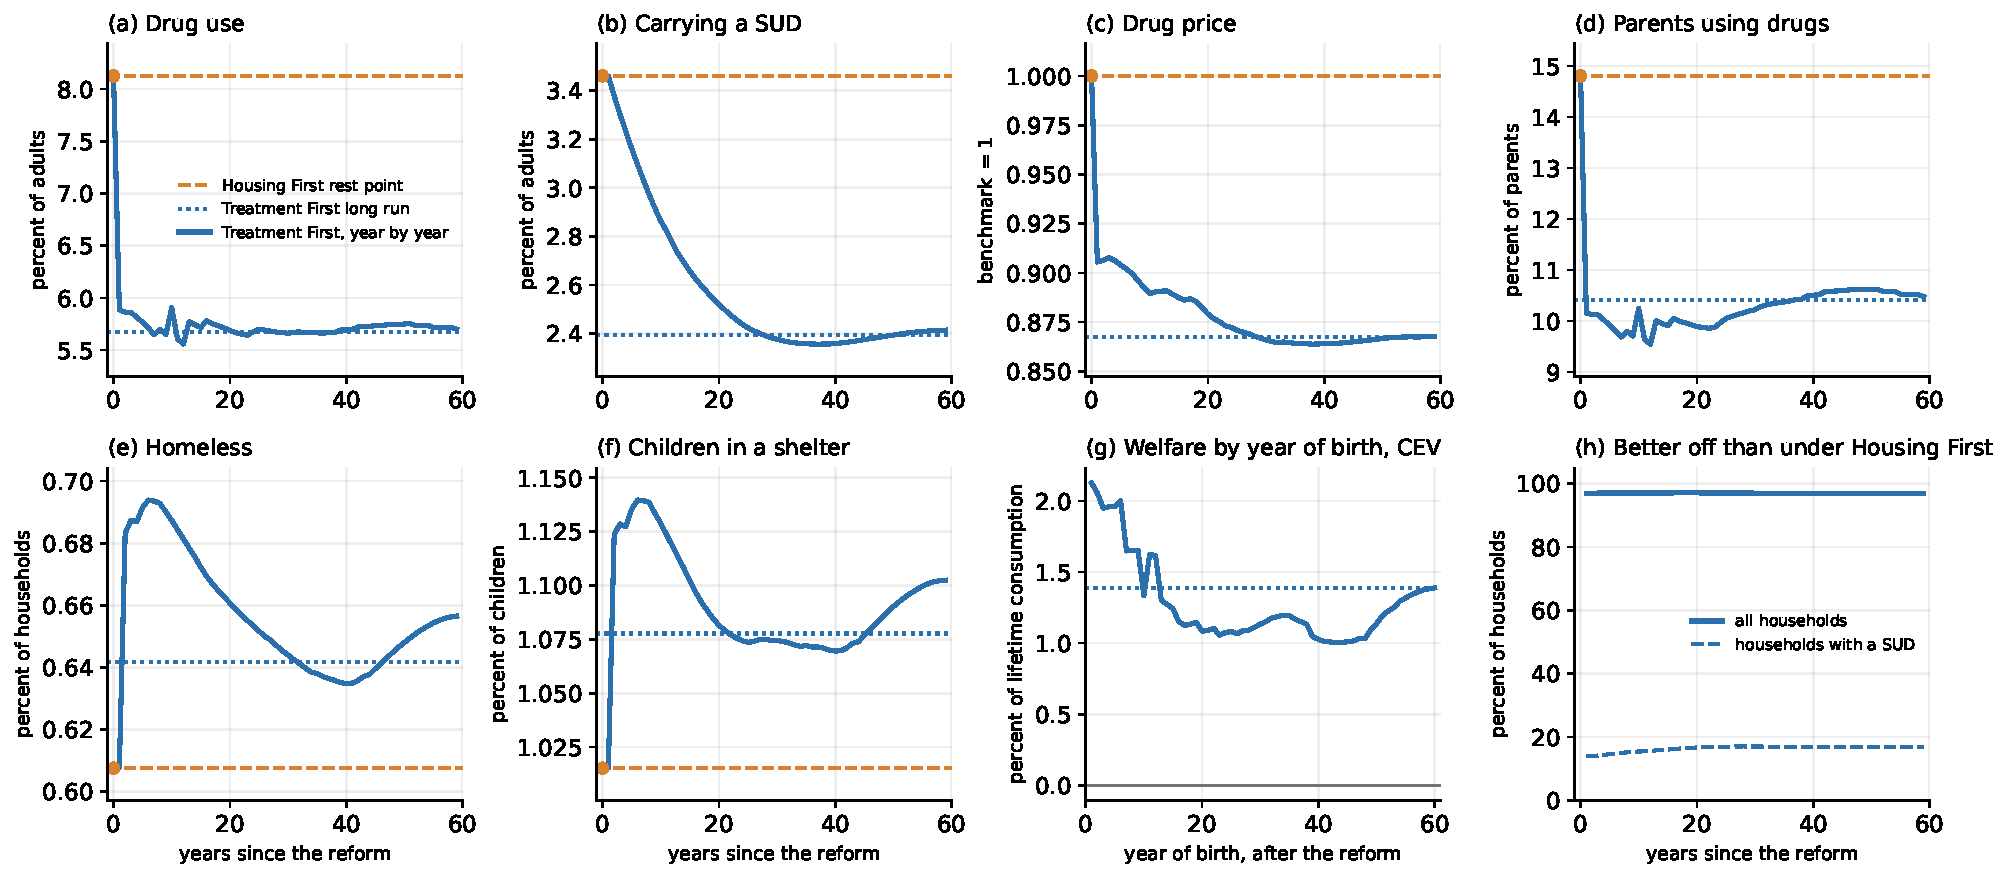
\includegraphics[width=\textwidth]{figures/full_transition.pdf}
\caption{The transition from Housing First to Treatment First, quantitative model}\label{fig:ftrans}
\notes{\textwidth}{Notes: panels (a) to (f) and (h) are by year since the reform, which lands at
the start of year 1, with the benchmark as year 0; the dashed orange line is the Housing
First benchmark, the dotted blue line the Treatment First long run and the solid blue line
the path. In panel (h) the dashed line is the share of households with a SUD who are worse off. Children are those of households aged 26 to 50. Panel (g) is the CEV of each cohort
born on the path, against the benchmark, by its year of birth. Panel (h) is the share of households worse off in each year of the path than in the
same state under Housing First, weighted by the benchmark's distribution.}
\end{figure}

Panels (a) and (d) show drug use and the share of parents who use, respectively. Drug use falls on impact: \updnum{$81$} percent of its long-run fall happens in
the first year. In the first year, the share of parents using drugs falls from \updnum{$16.35$} to \updnum{$13.57$} percent, \updnum{above} its long-run level of \updnum{$13.24$} percent. \updnum{It stays above its long-run level until year 12, because it counts the parents who have a SUD when the reform lands, whose number falls only slowly (panel (b)). From then on it moves around its long-run level.} The screen affects the decisions to go to treatment and to use drugs, both directly and through expectations. A voucher holder that uses risks losing its voucher within a year, and a household that uses risks having a voucher offer revoked later, when it may need one but have a SUD, since a disorder takes years to clear.

Panel (b) shows the
share with a SUD. This share falls gradually, because recovery is slow: half of its
long-run fall is done by year \updnum{$11$}, and nine tenths by year
\updnum{$27$}. The households that still have a SUD keep demand for the drug up, and the drug price stays
above its long-run level for \updnum{$33$} years (panel (c)). The elevated price deters
households without a SUD, at every age: in the first decade the number of drug users without
a SUD falls by up to \updnum{$23$} percent, against $18$ percent in the
long run. 

Panels (e) and (f) show homelessness and the share of children in a shelter, respectively. Neither rises at any point. Homelessness falls from \updnum{$0.62$} percent of households to \updnum{$0.60$} percent by year 10 and \updnum{$0.55$} percent by year \updnum{$60$}, against \updnum{$0.55$} percent in the long run, and the share of children in a shelter falls from \updnum{$1.03$} to \updnum{$1.00$} percent by year 10 and \updnum{$0.92$} percent by year \updnum{$60$}, against \updnum{$0.92$} percent in the long run. Both could have risen, since the households that have a SUD when the reform lands face losing their vouchers unless they enter treatment and stay sober. They do not, for three reasons. First, few households lose their vouchers: one with a SUD keeps its voucher by entering treatment and not using, and the screen catches a user with a probability of only $20$ percent a year, so at most \updnum{$0.13$} percent of households are excluded from the programme in any year. Second, drug use falls from the first year (panel (a)), so households spend less on drugs and have more left over to house themselves, and fewer acquire a SUD and experience longer unemployment. \updnum{Third, after the first three years, when it is as low as $6.55$ percent, $\pi_V$ stays above its Housing First level of $6.75$ percent, so the vouchers the screen frees go to other low-income households.}

Panel (g) shows the CEV of each cohort by its year of birth. Children born at the reform gain \updnum{$1.45$} percent of lifetime consumption, less than the \updnum{$2.57$} percent of those born in the long run, for two reasons. First, they grow up while the share of households with a SUD is still close to its Housing First level, since it falls only as fast as recovery allows: from \updnum{$3.83$} to \updnum{$3.47$} percent in the first ten years, against \updnum{$3.08$} percent in the long run.  This means that more children grow up with a parent who has the disorder, and more children enter their adult life with a lower productivity due to the earnings penalty. Second, $\pi_V$ is lower in the first years than in the long run: between \updnum{$6.55$} and \updnum{$6.90$} percent in the first decade, against \updnum{$7.80$} percent. Part of what Treatment First adds to the budget is the taxes paid by adults who grew up without the earnings penalty, while those adults start working only $J_K$ years after the reform. Until then, their parents are less likely to draw a voucher. The gain rises towards its long-run level for children born later, whose parents were themselves born after the reform.

Of the adults alive at the reform, only \updnum{$11$} percent are worse off under it, and even of those who have a SUD when it lands, \updnum{$33$} percent benefit, because the lower drug
price more than offsets the loss from the sobriety requirement for some of them. \updnum{Panel (h) repeats the comparison in every period of the path, with households in each state weighted as under Housing First. The share worse off stays between $2$ and $11$ percent, and the share of those with a SUD who are worse off falls from $67$ to $50$ percent as the price comes down further. Of the households entering adult life at 26, $33$ percent are better off in the first year, when $\pi_V$ is still close to its Housing First level, and $99.9$ percent by year 59.}

\subsection{Alternative transitions}\label{sec:alttrans}

The main transition lets a household with a SUD keep its voucher by entering treatment and not using. This section asks what the first periods of the reform look like when households with a SUD cannot stop using, so that only after recovery can they stay sober and pass the screen. I consider three alternatives, each with the screen catching every user or catching $20$ percent of users, and with the drug price and $\pi_V$ clearing every period. In the first, the screen applies from day one of the reform, and the disorder fails it whether or not the household is in treatment. In the second, the reform is announced, but Housing First continues for five periods and the same screen starts in period six. In the third, the same screen applies from the reform, but for its first five periods a household in treatment keeps its voucher even if it uses drugs. Table~\ref{tab:alttrans} shows how homelessness, the share of children in a shelter and the welfare of children born at the reform compare with the Housing First benchmark in each, beside the main transition (first row).

\begin{table}[!htb]\centering
\caption{The first years of the alternative transitions}\label{tab:alttrans}
\begingroup\small
\sbox{\ntbox}{\begin{tabular}{@{}lcccccc@{}}
\toprule
 & & \multicolumn{2}{c}{Homelessness} & \multicolumn{2}{c}{Children in a shelter} & Newborn's \\
\cmidrule(lr){3-4}\cmidrule(lr){5-6}
 & $p_{\mathrm{det}}$ & Largest rise & Periods above & Largest rise & Periods above & gain \\
\midrule
Main transition & 20 & none & none & none & none & 1.45 \\
\addlinespace
\multicolumn{7}{@{}l}{No exemption} \\
 & 100 & 13.6 (2) & 1--15 & 10.8 (2) & 2--11 & 6.57 \\
 & 20 & 5.4 (7) & 2--17 & 3.1 (5) & 2--11 & 3.09 \\
\addlinespace
\multicolumn{7}{@{}l}{Announced five periods ahead} \\
 & 100 & 7.3 (9) & 7--16 & 3.6 (9) & 7--12 & 4.54 \\
 & 20 & 3.4 (12) & 7--19 & 0.9 (11) & 8--13 & 1.92 \\
\addlinespace
\multicolumn{7}{@{}l}{Sobriety while in treatment exempt for the first five periods} \\
 & 100 & 5.2 (7) & 7--14 & 1.7 (7) & 7--10 & 6.24 \\
 & 20 & 1.6 (11) & 9--16 & none & none & 2.87 \\
\bottomrule
\end{tabular}}
\usebox{\ntbox}
\tabnote{Notes: Each row is a transition from the Housing First benchmark to Treatment First with the drug price and $\pi_V$ clearing every period, against Housing First's steady state. Main transition: Section~\ref{sec:ftrans}, where a household with a SUD keeps its voucher by entering treatment and not using. In the other rows it cannot stop using, and the disorder fails the screen even in treatment: from the reform (no exemption), from period six with Housing First until then (announced five periods ahead), or from period six with treatment alone passing it until then (sobriety while in treatment exempt for the first five periods). $p_{\mathrm{det}}$ is the detection rate, in percent. Largest rise: the largest percent increase over the first fifteen periods, with its period in brackets. Periods above: the periods in which it is above Housing First. Children in a shelter is the homelessness of households aged 26 to 50. Newborn's gain: the CEV of children born at the reform, percent of lifetime consumption. When every user is caught, no drug price clears the long-run drug market, because drug use jumps as the price moves through the level that would clear it; those transitions end at the long-run solution that comes closest.}
\endgroup
\end{table}



In the first alternative, how much the screen catches decides what happens along the way. Catching every user lowers homelessness by $30$ percent and the share of children in a shelter by $31$ percent in the long run, but it puts every voucher holder with a SUD out at once: homelessness rises by up to $14$ percent and the share of children in a shelter by up to $11$ percent, and they stay above their Housing First levels for $15$ and $11$ years, respectively, because $\pi_V$ rises only as the savings accrue. Catching only one in five users lowers both in the long run too, homelessness by $11$ percent and the share of children in a shelter by 11 percent, but it also raises them in the first years, though by less, because it puts fewer households out at once:  homelessness rises by up to $5$ percent and the share of children in a shelter by up to $3$ percent. Even so, children born at the reform gain $6.57$ percent of lifetime consumption when every user is caught and $3.09$ percent when $20$ percent are, against $1.45$ percent in the main transition. They gain more because the screen deters more: a household with a SUD cannot stop using, so the disorder costs it its voucher until it recovers, while in the main transition the household keeps the voucher by entering treatment and not using. By period ten, $2.80$ percent of households have a SUD when every user is caught and $3.24$ percent when $20$ percent are, against $3.47$ percent, so fewer of these children grow up with a parent who has the disorder, and $\pi_V$ is higher throughout their childhood.

Announcing the screen five periods before it starts lowers the rise but does not eliminate it. While Housing First continues, households cut their drug use at once in anticipation of a screen that will catch every user, by \del{$30$} \new{$29$} percent in the first period, and homelessness and the share of children in a shelter fall below their Housing First levels. Once it starts revoking vouchers, they rise by up to $7$ and $4$ percent, against $14$ and $11$ percent without the announcement. When it catches one in five users, they rise by up to $3$ and $0.9$ percent. Children born at the reform gain \del{$4.62$} \new{$4.54$} percent of lifetime consumption when every user is caught and $1.92$ percent when one in five users are. The first is less than the $6.57$ percent without the announcement, because $\pi_V$ does not rise until the screen starts and drug use falls by less in the first period than the $40$ percent when the screen starts at once.

Exempting sobriety while in treatment for the first five periods lets a household with a SUD keep its voucher in those periods by entering treatment, even if it uses drugs, and more households do: $36$ percent of those with a SUD are in treatment, against $25$ percent under Housing First. When the screen catches one in five users, homelessness stays below its Housing First level for the first eight periods but rises above it by at most $1.6$ percent after the exemption ends, and the share of children in a shelter never rises above its Housing First level. When every user is caught, homelessness stays below its Housing First level for the first six periods but rises above it by at most \del{$5.0$} \new{$5.2$} percent after the exemption ends, and the share of children in a shelter by at most \del{$1.3$} \new{$1.7$} percent. Children born at the reform gain $2.87$ percent of lifetime consumption when one in five users are caught, more than the $1.45$ percent in the main transition, although the screen catches one in five users in both. Here a household with a SUD cannot stop using, so once the exemption ends the disorder puts its voucher at risk until it recovers, while in the main transition the household keeps the voucher by entering treatment and not using. Starting to use therefore risks more, and fewer households use drugs: by period ten, $3.27$ percent of households have a SUD, against $3.47$ percent, so fewer of these children grow up with a parent who has the disorder, and $\pi_V$ is higher throughout their childhood. When every user is caught, they gain \del{$6.37$} \new{$6.24$} percent.

%======================================================================
\section{Discussion and implications}\label{sec:discussion}

To close, I return to the question I started with: should housing assistance require sobriety?   I argue that the answer is  ``Yes'' if the externalities on children are counted but ``No'' if the moral hazard argument is invoked, which is the argument that dominates the policy debate.   Specifically, I show that although, in an economy without the externalities on children, Treatment First cuts drug use by $28$ percent, a newborn is still worse off, because the screen takes away an option from households that weigh the risks correctly, while the budget gives back less than the screen takes.

 I  then demonstrate that drug use takes away consumption and housing from children and reduces their productivity as adults.  But because a parent counts only the share $\omega_c$ of these costs, the deterrence the screen creates generates more gain to the child than cost to the parent, and welfare rises. With the drug price and $\pi_V$ held, the parents lose $1.19$ percent of their own lifetime consumption, about what they lose without the externalities, while a newborn gains $2.82$ percent, so the reform raises welfare on net once the children are counted. With the budget rebalanced and the drug price clearing, as they would be after a real reform, Treatment First cuts drug use by $21$ percent, lowers homelessness by $11$ percent, and raises a newborn's welfare by $2.57$ percent of lifetime consumption, three quarters of it an externality its parent does not count. Once general-equilibrium effects are accounted for, the parents gain too, because the higher $\pi_V$ and the cheaper drug outweigh the option the screen removes. Along the transition, neither homelessness nor the share of children in a shelter rises, and children born at the reform gain \updnum{$1.45$} percent.

Three lessons follow. First, the arguments for Housing First and Treatment First made by different advocacy
groups leave out the outcome that matters most: what happens to the children of the households a sobriety requirement deters from using, in what they consume while living with their parents, in whether they become homeless and in what they earn as adults.

Second, the model agrees with the micro evidence behind Housing First on the households it follows: housing, and a sobriety condition on it, raise the recovery of households with a SUD by about as much as in the trial that measures both, and losing a voucher raises the mortality of households with SMI by about as much as Housing First lowers it among homeless veterans with mental illness. As that evidence implies, those with a SUD lose from Treatment First: with the drug price and $\pi_V$ held, as in a trial, which is too small to move either, $74$ percent of those who have one when the reform lands are worse off, and even once both clear, \updnum{$67$} percent are. The macro effects the trials do not capture, however, overturn the conclusions. The trials follow only households already in a bind: adults who are homeless, most with SMI and many with a SUD. They do not follow the households that could get into a bind but that the condition deters from starting to use drugs. Nor do they observe the vouchers the condition's savings buy for others, or the children's adult lives. Once those are counted, aggregate homelessness and childhood homelessness drop and welfare increases.

Third, homelessness and childhood homelessness do not fall along the transition if treatment and sobriety are not a real option for the households that already have a SUD. A temporary exemption for those with a SUD keeps the latter from ever rising and the former's rise small: if a household in treatment keeps its voucher, sober or not, for the first five periods, and the screen catches one in five users, the share of children in a shelter never rises above its Housing First level and homelessness rises by at most $1.6$ percent, with newborns gaining even more than in the main transition.

\clearpage
\appendix
\setcounter{table}{0}\renewcommand{\thetable}{A\arabic{table}}
\section[Calibration of the standard parameters]{Calibration of the standard parameters}\label{sec:stdparams}

  My full calibration contains many parameters, many of which are more conventional and used in many papers. Here, I show how I set those thirty-three parameters. I calibrate six of them internally and set the other twenty-seven externally from estimates in the literature or from statute. Table~\ref{tab:stdparams} and the entries below proceed in the same seven blocks. In each entry, I give the moment or source that pins down the parameter and the value of that moment in the data. For the internally calibrated parameters, the Model column also presents the model's performance.

 None of these parameters are inert. They too matter for the experiments, but they are more standard and matter less for the results than the parameters that I covered in the main text. For instance, the discount factor affects how much weight households give to dying in a later period. The dispersion of productivity determines how many households are poor enough to be willing to risk having a disorder, and risk aversion determines how much households value the insurance of housing assistance.

\begin{table}[htbp]\centering
\caption{Standard parameters}\label{tab:stdparams}
\begingroup\scriptsize\setlength{\tabcolsep}{3pt}
\begin{tabular}{@{}lL{3.6cm}cL{5.5cm}rrr@{}}
\toprule
Parameter & Description & Set & Moment and source & Data & Model & Value \\
\midrule
\multicolumn{7}{@{}l}{\textcolor{red}{\emph{Preferences}}} \\
$\sigma$ & Risk aversion & Ext. & Attanasio and Weber (2010) & 2.00 & n.a. & 2.00 \\
$\gamma$ & CD weight on housing & Int. & Renters above 30 pct of income, ACS 2023 & 49.7\% & \textemdash & \textemdash \\
$\beta$ & Discount factor & Int. & Wealth over output, BEA fixed assets & 3.00 & \textemdash & \textemdash \\
\textcolor{red}{$\omega_{\ell}$} & \textcolor{red}{Weight on leisure} & \textcolor{red}{Int.} & \textcolor{red}{Average hours worked, Guvenen et al.\ (2023)} & \textcolor{red}{0.40} & \textemdash & \textemdash \\
\addlinespace
\multicolumn{7}{@{}l}{\textcolor{red}{\emph{The rental ladder}}} \\
$\underline h$ & Smallest rental size & Int. & Share in smallest unit size, ACS 2023 & 13.2\% & \textemdash & \textemdash \\
$\bar h$ & Largest rental size & Int. & Share in largest unit size, ACS 2023 & 62.7\% & \textemdash & \textemdash \\
$\varsigma$ & Curvature of the ladder & Ext. & Set; the two ends carry the distribution & 1.80 & n.a. & 1.80 \\
\addlinespace
\multicolumn{7}{@{}l}{\textcolor{red}{\emph{Earnings and employment}}} \\
$\varepsilon(j)$ & Age profile of efficiency & Ext. & Quadratic in age, PSID and CPS hump & profile & n.a. & profile \\
$\rho_y$ & Persistence of log prod. & Ext. & Storesletten et al.\ (2004) & 0.90 & n.a. & 0.90 \\
$\sigma_y$ & Dispersion of log prod. & Ext. & Storesletten et al.\ (2004) & 0.20 & n.a. & 0.20 \\
$\bar\pi^{eu}$ & Job separation rate & Int. & Unemployment rate, BLS CPS 2014--24 & 4.85\% & \textemdash & \textemdash \\
$\bar\pi^{ue}$ & Job finding rate, annual & Ext. & Krueger, Cramer and Cho (2014) & 0.55 & n.a. & 0.55 \\
\addlinespace
\multicolumn{7}{@{}l}{\textcolor{red}{\emph{Survival and mental illness}}} \\
$\bar\phi(j)$ & Baseline survival by age & Ext. & SSA period life table, ages 26 to 85 & profile & n.a. & profile \\
$p_m$ & Age profile of SMI prevalence & Ext. & Share with SMI, NSDUH 2023 & 5.5\% & n.a. & 5.5\% \\
\addlinespace
\multicolumn{7}{@{}l}{\textcolor{red}{\emph{Interest, taxes and public spending}}} \\
$r$ & Risk free rate & Ext. & Kaplan, Mitman and Violante (2020) & 0.03 & n.a. & 0.03 \\
$\xi$ & Tax progressivity & Ext. & Heathcote et al. (2017) & 0.85 & n.a. & 0.85 \\
$\tau_k$ & Capital income tax & Ext. & US long run rate on gains and dividends & 0.15 & n.a. & 0.15 \\
$\tau_{\ell}$ & Tax level & Ext. & Clears the government budget & in eqm. & n.a. & in eqm. \\
$G$ & Other public spending & Ext. & Residual at benchmark, then held fixed & in eqm. & n.a. & in eqm. \\
\addlinespace
\multicolumn{7}{@{}l}{\textcolor{red}{\emph{Transfers and the voucher rule}}} \\
$\psi$ & UI replacement rate & Ext. & DOL statutory replacement rates & 0.50 & n.a. & 0.50 \\
$\bar y$ & Cap on insurance earnings & Ext. & DOL state benefit maxima & 1.00 & n.a. & 1.00 \\
$\kappa_V$ & Voucher eligibility cutoff & Ext. & HUD rule & 0.50 & n.a. & 0.50 \\
$\kappa_r$ & Tenant contribution rate & Ext. & HUD rule & 0.30 & n.a. & 0.30 \\
\addlinespace
\multicolumn{7}{@{}l}{\textcolor{red}{\emph{The drug market}}} \\
$j_E$ & Last experimentation age & Ext. & Reported with and without it & 55 & n.a. & 55 \\
\textcolor{red}{$\nu_1$} & \textcolor{red}{Drug supply shifter} & \textcolor{red}{Ext.} & \textcolor{red}{Normalisation, so $p_v=1$} & \textcolor{red}{norm.} & \textcolor{red}{n.a.} & \textcolor{red}{norm.} \\
\textcolor{red}{$p_v$} & \textcolor{red}{Price of drugs} & \textcolor{red}{Ext.} & \textcolor{red}{Clears the drug market in the benchmark} & \textcolor{red}{1.00} & \textcolor{red}{n.a.} & \textcolor{red}{1.00} \\
\bottomrule
\end{tabular}
\notes{\textwidth}{Note: n.a.\ in the Model column marks a parameter that is set from outside rather than calibrated inside the model. For those the model produces no internal target to compare with the data, so the cell reads n.a.\ rather than a dash, which keeps them distinct from the internally calibrated parameters.}
\endgroup
\end{table}



\paragraph{Block 7: Preferences.}  The four parameters in this block determine what households care about and what they are willing to give up in exchange.
\begin{description}\setlength{\itemsep}{0.25em}\setlength{\parskip}{0em}
\item[$\sigma$, risk aversion.]  The risk-aversion parameter shapes the marginal utility of consumption, and through it, it affects the welfare comparisons in the experiments in this paper. When it is increased, households prefer smoother consumption, and therefore housing assistance as insurance is worth more to them. I set it to the standard value of two, following
Attanasio and Weber (2010).
\item[$\gamma$, the weight on housing services.] It is the weight on housing in the
bundle of consumption and housing, so it sets what a dwelling is worth against
consumption, and that bundle is what the drug is weighed against. As
$\gamma$ rises housing is worth more relative to consumption, households buy more of it,
and the share of spending that goes on housing rises with it. $\gamma$ is chosen for the share
it produces: shelter plus utilities take $26.8$ percent of expenditure in the 2024 Consumer Expenditure Survey (CEX), which excludes illicit drug spending.
\item[$\beta$, the discount factor.] It sets how much households discount the
future, and thus how much they save and how much the prospect of death deters them from using drugs. As it rises households save more, the
 wealth-to-output ratio rises and households are more deterred by death. It is chosen so that wealth over output
matches the national accounts, a ratio of three, from the Bureau of Economic Analysis (BEA) fixed asset tables
against National Income and Product Accounts (NIPA) output, both read at the 2023 vintage, the last year the fixed asset tables cover.
\item[$\xi(j)$, the equivalence scale.] The household's consumption and
dwelling are shared with the child while it lives with its parent, and thus are divided by
$\xi(j)$ to give what each member gets. Raise it and each member gets less of a given budget, and the child counts for more of the household, through the weight $\xi(j)-1$ in~\eqref{eq:futil}. It is the square-root scale (OECD, 2013), $\sqrt{N(j)}$, where $N(j)$ in the model is set to two while
the child lives with the parent ($j\le J_K$), from the parent's age 26 to 50, and to one after the child has left ($j>J_K$).
\end{description}

\paragraph{Block 8: Rental ladder.} These three parameters build the grid of dwelling
sizes a household chooses from. Below the smallest rung is the shelter, $h_1$, which was calibrated in Block 2.
\begin{description}\setlength{\itemsep}{0.25em}\setlength{\parskip}{0em}
\item[$h_2$, the smallest rental size.]   The size of the smallest dwelling is what determines how much of its income a poor household has to spend to avoid homelessness. When the smallest dwelling is larger, it is more expensive to rent, and thus more households are cost burdened and more likely to become homeless, and a voucher is worth more to them. It is chosen so that
the fraction of renters paying more than half of their income for housing is similar to
the data, $19.2$ percent in the 2022 SCF; the model gives $25.8$
percent.
\item[$h_3/h_2$ and $h_4/h_2$, the spacing of the ladder.]   The two ratios here determine the amount of housing services obtained by renting the middle and largest dwelling options. Therefore, they affect what a household that can afford more than the smallest unit can rent. Larger ratios make each step up the ladder cost more to rent, and thus fewer households can afford the larger options. The two larger
rungs are set at $4.00$ and $8.00$ times the smallest.
\end{description}

\paragraph{Block 9: Earnings and employment.}   This block has eleven parameters that govern the maximum periods of life a household can live, until what age it works, and what it can expect to earn while it is of working age. These parameters also set how persistent and frequent shocks to employment and productivity are.
\begin{description}\setlength{\itemsep}{0.25em}\setlength{\parskip}{0em}
\item[$J$, $J_K$ and $J_R$, the length of life, of child rearing and of working life, respectively.] A household lives at most
$J$ periods, has its child at home for its first $J_K$ of them and works until model age $J_R$, after which it retires on social security.
  $J$ and $J_R$ set the maximum number of years a household can live and work, respectively, and $J_K$ sets how long a parent's drug use reaches its child, since the child lives with it during those $J_K$ years. A higher $J$ or $J_R$ makes a disorder that shortens life or employment more costly, whereas a higher $J_K$ makes the budget and childhood homelessness externalities last longer. I set $J=60$, so
that with $j=1$ at age 26 the last age is $85$, $J_K=25$, so that the child lives at home while its parent is 26 to $50$, and $J_R=41$, so that retirement begins at age $66$, the
full retirement age under social security for those born between 1943 and 1954.
\item[$\varepsilon(j)$, the age profile of efficiency.] This is the deterministic hump in
earnings over the life cycle. Without it every
household with the same productivity would earn the same at every age, and the ages at which households are
poor, and so at risk of homelessness and of using, would be wrong at both ends of
working life. I take it as the exponential of a quadratic in age used by
Greenwood et al.\ (2025), $\varepsilon(j)=\exp\{-(j-1)^2/1800+(j-1)/30\}$ with $j=1$
at age $26$. It peaks at age $56$, having risen $65$ percent from age $26$, and then
falls $4$ percent from the peak to age $65$, the last working age.

\item[$\rho_y$ and $\sigma_\zeta$, the productivity process.] Log
productivity is persistent but not permanent: it follows an autoregressive process
with persistence $\rho_y$ and shocks with standard deviation
$\sigma_\zeta$. $\sigma_\zeta$ is what decides how many households are poor
enough to be at risk of homelessness, and the share of earnings
that goes to the bottom half of working households falls as it rises. I set
$\rho_y=0.90$, the persistence of the income process in Guvenen et al.\ (2023). $\sigma_\zeta$
is calibrated to the bottom half's share of earnings among households aged 26 to 65 with
positive wage income in the 2022 SCF, $17.2$ percent.

\item[$\rho$, the persistence of productivity across generations.] The
child's log productivity at entry into adulthood is drawn around its parent's with weight $\rho$ and
around the mean with weight $1-\rho$, so $\rho$ is how much of its parent's current productivity a
child keeps. It is the channel through which anything that lowers a parent's productivity lowers its child's: a parent whose own productivity carries the penalty $\delta_d$, because its own parent had a SUD, also passes a lower draw on to its child, so a
parent's SUD lowers productivity beyond the next generation. Raise it and a child's prospects depend more
on its parent's decisions, and the \emph{earnings externality} grows. It is set
externally at $0.50$, between the intergenerational elasticities of earnings
in Solon (1992) and Mazumder (2005).
\item[$\bar\pi^{eu}$, the job separation rate.] This parameter determines the chance that an employed household
loses its job each year. It is scaled by $\varpi(y)$ in~\eqref{eq:femp}, so separations are likelier at low
productivity. Raise it and more households lose work each year, so the unemployment
rate rises with it. It is chosen to reproduce the aggregate
unemployment rate in the Current Population Survey (CPS) of the Bureau of Labor Statistics (BLS) over 2014 to 2024,
$4.9$ percent, given the job-finding rate set externally below.
\item[$\varpi(y)$, separations by productivity.] This parameter tilts the separation rate across
productivity, so that low-productivity households lose their jobs more often, which is what
puts them at a higher risk of homelessness.   A steeper gradient exposes low-productivity households to a higher chance of unemployment, and thus a higher risk of homelessness. It is normalised to average one across households, so
that $\bar\pi^{eu}$ alone sets the aggregate unemployment rate. Each productivity node takes the
unemployment odds of the education group it falls in, from the BLS 2019 annual averages of
unemployment by educational attainment for ages 25 and over, with the education groups ordered along productivity by their median earnings.
\item[$\bar\pi^{ue}$, the annual job-finding rate.] This parameter is the probability that an
unemployed household finds work each year it is unemployed. With the divisors $\kappa^{ue}_{d}$ and $\kappa^{ue}_{m}$ it sets how long an unemployed household with a SUD or SMI is expected to remain unemployed.  When it is raised, unemployment spells are shorter on average, and thus fewer households are unable to pay rent and become homeless. I set it to
$0.55$ from the annual exit rate Krueger et al.\ (2014) estimate on
matched CPS panels.
\item[$p_{ui}$, the share of separations that receive UI.] A household that
loses its job draws UI for one year with probability $p_{ui}$ and nothing
otherwise. It sets how many of the newly unemployed fall straight to zero
earnings, and how costly being unemployed is. I set it to $0.30$, since in the BLS supplement to the CPS for 2022 about seven in ten unemployed people who worked in the past year did not apply for UI after losing their job.
\end{description}

\paragraph{Block 10: Baseline survival and SMI onset.} These two parameters are the survival and
the SMI-onset age profiles.
\begin{description}\setlength{\itemsep}{0.25em}\setlength{\parskip}{0em}
\item[$\bar\phi(j)$, baseline survival by age.] This is the baseline chance of surviving to the
next age, before any multiplier. It is the base that every mortality multiplier in Section~\ref{sec:fullcal}, for a SUD, homelessness and SMI, scales. Raise it and households expect to live longer, so the life a SUD puts at risk is worth more. I take the profile from the life table for the total population of the United States in 2010 (Arias, 2014), for ages $26$ to $85$.

\item[$\varsigma_m(j)$, the age profile of SMI onset.] This determines the shape of onset
across ages, normalised to one at age $26$, so that $\omega_m$ in Table~\ref{tab:eleven} sets its
level alone. It is here rather than in Table~\ref{tab:eleven} because, like the age survival profile, it only sets the
baseline. What actually affects the impact of Housing First versus Treatment First is $\iota$, the multiplier a SUD puts
on SMI onset, which is in Table~\ref{tab:eleven}. It is the onset that
reproduces a log-linear fit to the share of adults carrying SMI at each age in NSDUH
2024.
\end{description}

\paragraph{Block 11: Interest and taxes.}
\begin{description}\setlength{\itemsep}{0.25em}\setlength{\parskip}{0em}
\item[$r$, the risk-free rate.] This parameter sets the return on saving.   A higher interest rate improves the return on savings, and thus households accumulate more assets, which help cushion them during spells of unemployment. I set it to three percent, from Kaplan et al.\
(2020).

\item[$\varphi$, tax progressivity.] This is the exponent on income in the tax schedule of
Section~\ref{sec:ftaxes}, and it determines the progressivity of the labour income tax.   When its value is lower, the tax system becomes more progressive. In that case, households with low incomes keep more of what they earn. It is set to $0.85$, in line with Heathcote et al.\ (2017). 

\item[$\tau_{\ell}$, the scale of after-tax labour income.] Given $\varphi$, this parameter sets how much
of their labour income households keep after tax on average, so raising it lowers the tax liability. It does not move in the experiments: the budget is
balanced by $\pi_V$ instead. It is calibrated to
an average labour income tax rate of $22.4$ percent,
which is what McDaniel (2007) measures for the United States and what Guvenen et al.\ (2023) use.

\item[$\tau_k$, the capital income tax rate.] This parameter affects the after-tax return on savings.   A higher capital income tax rate reduces the after-tax return to savings, and this discourages households from saving. I set it to fifteen percent, consistent
with the statutory United States rate on long-term capital gains and qualified
dividends for the middle of the income distribution, which the Internal Revenue
Service (IRS) sets out in Topic 409
(\url{https://www.irs.gov/taxtopics/tc409}).

\end{description}

\paragraph{Block 12: Social security benefits and programmes' rules.}
\begin{description}\setlength{\itemsep}{0.25em}\setlength{\parskip}{0em}
\item[$S(y)$ and $\underline S$, social security and its floor.] Retirement income follows the statutory
primary insurance amount: it replaces a share of the household's income at its last working
age, a share that falls at each of the two bend points of the Social Security Administration (SSA), up to
the taxable maximum, with the SSI payment as a floor (the full function is detailed in footnote~\ref{fn:ss}). As $S(y)$ rises the old are richer, so the value of a life
still to be lived rises and with it the cost of a disorder that shortens it. The shares
$\alpha_1,\alpha_2,\alpha_3$ are $0.90, 0.32, 0.15$ below the first bend point, between the two and above the second, respectively. The
bend points $k_1$ and $k_2$ and the taxable maximum $y^{\max}$ are the SSA's 2024 dollar
amounts divided by its average wage index, $0.22$, $1.33$ and
$2.64$, respectively. The floor, $\underline S$, is $0.18$ of average
labour income.
\item[$\psi_{ui}$ and $\bar y$, UI.]   The first parameter here sets the UI replacement rate, while the second parameter caps the earnings on which UI is paid. Raising either makes the first year out of work less costly for a household who lost their job, and thus makes it less likely that a household would end up in a shelter. I set them to fifty percent and one
times average labour income, respectively, taking both from the statutory replacement rates
and state benefit maxima that the Department of Labor compiles in its comparison of
state UI laws
(\url{https://oui.doleta.gov/unemploy/statelaws.asp}).

\item[$\kappa_V$ and $\kappa_r$, the voucher rules.] These two set the income
cutoff for eligibility and the tenant's rent contribution, respectively. Raise $\kappa_V$ and more households are eligible, so more have a voucher to lose under Treatment First; raise $\kappa_r$ and a voucher pays less, so losing one costs less. I take both from HUD's own
rules: half of median income and thirty
percent, respectively. The first is the very low-income limit HUD publishes
annually with its income limits
(\url{https://www.huduser.gov/portal/datasets/il.html}); the second is the share of its before-tax income a tenant pays towards the rent, the voucher
paying the rest up to the payment standard, under the Housing Choice
Voucher programme
(\url{https://www.hud.gov/helping-americans/housing-choice-vouchers}).

\item[$\varrho$, the food stamp clawback rate.] This is the rate at which food assistance is withdrawn as income rises. Raise it and food assistance is clawed back faster, so it stops at a lower income and pays less to every household that still receives it. I set it to thirty percent, which is the statutory rule (7 CFR 273.10).
\end{description}

\paragraph{Block 13: Drug market.} The two parameters in this block describe the rest of the drug
market of Block 6. The first, $J_E$, fixes who can enter the market (footnote~\ref{fn:je}); the second is set so that supply equals demand in the benchmark, and is
then held fixed.
\begin{description}\setlength{\itemsep}{0.25em}\setlength{\parskip}{0em}
% THE PARENTHETICAL BELONGS IN THE BODY, NOT THE LABEL. A description
% label does not wrap: it is typeset on one line and runs off the page,
% which is what it did here.

\item[$J_E$, the last age at which use can begin.] This parameter is the last age at which a household without a SUD can start using; one that already has a SUD at that age can keep using. It decides who can enter the drug market, and so how many households a policy that deters use can reach. As it rises, more old households can start using at little cost, since too little life remains for the disorder to damage (footnote~\ref{fn:je}), and the model produces too much old-age use. I set it to model age $55$, the equivalent of age $80$ when the model runs to age $85$.

\item[$\nu_1$, the supply shifter.] A pure normalisation, chosen so that supply
equals demand at $p_v=1$ in the benchmark, and kept fixed across experiments, in which the price is free to adjust. It normalises units, not behaviour.

\end{description}

\clearpage


\section*{References}



{\normalsize
\setlength{\parindent}{0em}
\begin{list}{}{\setlength{\leftmargin}{1.5em}\setlength{\itemindent}{-1.5em}\setlength{\itemsep}{0.35em}\setlength{\parsep}{0em}}
\item Abbott, B., G. Gallipoli, C. Meghir and G. L. Violante (2019). ``Education Policy and Intergenerational Transfers in Equilibrium.'' \emph{Journal of Political Economy} 127(6), 2569--2624.
\item Abramson, B. (2026). ``The Equilibrium Effects of Eviction Policies.'' \emph{Journal of Finance}, published online, \url{https://doi.org/10.1111/jofi.70046}.
\item AFCARS. \emph{Adoption and Foster Care Analysis and Reporting System}, US Department of Health and Human Services, Administration for Children and Families, FY2017 release.
\item Altonji, J., F. Hayashi and L. Kotlikoff (1997). ``Parental Altruism and Inter Vivos Transfers: Theory and Evidence.'' \emph{Journal of Political Economy} 105(6), 1121--66.
\item Arias, E. (2014). ``United States Life Tables, 2010.'' \emph{National Vital Statistics Reports} 63(7). Hyattsville, MD: National Center for Health Statistics.
\item {\AA}sb{\o}, G. et al.\ (2022). ``The Time Is Ripe for a Consensus Definition of Clinical Recovery in First-Episode Psychosis: Suggestions Based on a 10-Year Follow-Up Study.'' \emph{Schizophrenia Bulletin} 48(4), 839--49.
\item Attanasio, O. P. and G. Weber (2010). ``Consumption and Saving: Models of Intertemporal Allocation and Their Implications for Public Policy.'' \emph{Journal of Economic Literature} 48(3), 693--751.
\item Aubry, T. et al.\ (2016). ``A Multiple-City RCT of Housing First With Assertive Community Treatment for Homeless Canadians With Serious Mental Illness.'' \emph{Psychiatric Services} 67(3), 275--81.
\item Arrow, K. J. (1963). ``Uncertainty and the Welfare Economics of Medical Care.'' \emph{American Economic Review} 53(5), 941--973.
\item Balsa, A. I. (2008). ``Parental Problem-drinking and Adult Children's Labor Market Outcomes.'' \emph{Journal of Human Resources} 43(2), 454--486.
\item Barro, R. J. and G. S. Becker (1989). ``Fertility Choice in a Model of Economic Growth.'' \emph{Econometrica} 57(2), 481--501.
\item Bassuk, E. L., J. C. Buckner, L. F. Weinreb, A. Browne, S. S. Bassuk, R. Dawson and J. N. Perloff (1997). ``Homelessness in Female-Headed Families: Childhood and Adult Risk and Protective Factors.'' \emph{American Journal of Public Health} 87(2), 241--248.
\item Becker, G. S. and K. M. Murphy (1988). ``A Theory of Rational Addiction.'' \emph{Journal of Political Economy} 96(4), 675--700.
\item Becker, G. S., K. M. Murphy and M. Grossman (2006). ``The Market for Illegal Goods: The Case of Drugs.'' \emph{Journal of Political Economy} 114(1), 38--60.
\item Bradizza, C. M., P. R. Stasiewicz and N. D. Paas (2006). ``Relapse to alcohol and drug use among individuals diagnosed with co-occurring mental health and substance use disorders: A review.'' \emph{Clinical Psychology Review} 26(2), 162--78.
\item Burt, M. R., L. Y. Aron and E. Lee (2001). \emph{Helping America's Homeless: Emergency Shelter or Affordable Housing?} Washington, DC: Urban Institute Press.
\item Card, D. (1999). ``The Causal Effect of Education on Earnings.'' In O. Ashenfelter and D. Card (eds.), \emph{Handbook of Labor Economics}, vol.\ 3A, 1801--63. Amsterdam: Elsevier.
\item Caulkins, J. P. (2001). ``Drug Prices and Emergency Department Mentions for Cocaine and Heroin.'' \emph{American Journal of Public Health} 91(9), 1446--48.
\item Chetty, R., N. Hendren, P. Kline and E. Saez (2014). ``Where is the Land of Opportunity? The Geography of Intergenerational Mobility in the United States.'' \emph{Quarterly Journal of Economics} 129(4), 1553--1623.
\item Chetty, R., N. Hendren and L. Katz (2016). ``The Effects of Exposure to Better Neighborhoods on Children.'' \emph{American Economic Review} 106(4), 855--902.
\item Chyn, E. (2018). ``Moved to Opportunity: The Long-Run Effects of Public Housing Demolition on Children.'' \emph{American Economic Review} 108(10), 3028--56.
\item Conesa, J. C., S. Kitao and D. Krueger (2009). ``Taxing Capital? Not a Bad Idea after All!'' \emph{American Economic Review} 99(1), 25--48.
\item Costa, D.\ L.\ and M.\ E.\ Kahn (2004). ``Changes in the Value of Life, 1940--1980.'' \emph{Journal of Risk and Uncertainty} 29(2), 159--80.
\item Costantini, S. (2025). ``Housing First or Treatment First? Evidence from the VA's Homelessness Programs.'' Working paper, University of California, Berkeley.
\item Dahl, G. B. and L. Lochner (2012). ``The Impact of Family Income on Child Achievement: Evidence from the Earned Income Tax Credit.'' \emph{American Economic Review} 102(5), 1927--56.
\item Desmond, M. and C. Gershenson (2016). ``Housing and Employment Insecurity among the Working Poor.'' \emph{Social Problems} 63(1), 46--67.
\item Eide, S. (2020). ``Housing First and Homelessness: The Rhetoric and the Reality.'' Manhattan Institute.
\item Felitti, V. et al.\ (1998). ``Relationship of Childhood Abuse and Household Dysfunction to Many of the Leading Causes of Death in Adults.'' \emph{American Journal of Preventive Medicine} 14(4), 245--58.
\item Fudala, P. J. et al.\ (2003). ``Office-based treatment of opiate addiction with a sublingual-tablet formulation of buprenorphine and naloxone.'' \emph{New England Journal of Medicine} 349(10), 949--958.
\item Gallet, C. A. (2014). ``Can Price Get the Monkey Off Our Back? A Meta-Analysis of Illicit Drug Demand.'' \emph{Health Economics} 23(1), 55--68.
\item Goering, P. et al.\ (2014). \emph{National At Home/Chez Soi Final Report}. Mental Health Commission of Canada.
\item Greenwood, J., N. Guner and K. A. Kopecky (2025). ``The Downward Spiral: A Macroeconomic Analysis of the Opioid Crisis.'' Working paper.
\item Grossman, M. and F. Chaloupka (1998). ``The demand for cocaine by young adults: a rational addiction approach.'' \emph{Journal of Health Economics} 17(4), 427--74.
\item Gruber, J. and B. K\H{o}szegi (2001). ``Is Addiction `Rational'? Theory and Evidence.'' \emph{Quarterly Journal of Economics} 116(4), 1261--1303.
\item Gubits, D., M. Shinn, M. Wood, S. Bell, S. Dastrup, C. Solari, S. Brown, D. McInnis, T. McCall and U. Kattel (2016). ``Family Options Study: 3-Year Impacts of Housing and Services Interventions for Homeless Families.'' US Department of Housing and Urban Development, Office of Policy Development and Research.
\item Gubits, D., M. Shinn, M. Wood, S. R. Brown, S. R. Dastrup and S. H. Bell (2018). ``What Interventions Work Best for Families Who Experience Homelessness? Impact Estimates from the Family Options Study.'' \emph{Journal of Policy Analysis and Management} 37(4), 835--866.
\item Gutwinski, S., S. Schreiter, K. Deutscher and S. Fazel (2021). ``The prevalence of mental disorders among homeless people in high-income countries: An updated systematic review and meta-regression analysis.'' \emph{PLOS Medicine} 18(8), e1003750.
\item Guvenen, F., G. Kambourov, B. Kuruscu, S. Ocampo and D. Chen (2023). ``Use It or Lose It: Efficiency and Redistributional Effects of Wealth Taxation.'' \emph{Quarterly Journal of Economics} 138(2), 835--894.
\item Hall, R.\ E.\ and C.\ I.\ Jones (2007). ``The Value of Life and the Rise in Health Spending.'' \emph{Quarterly Journal of Economics} 122(1), 39--72.
\item Heathcote, J., K. Storesletten and G. Violante (2017). ``Optimal Tax Progressivity: An Analytical Framework.'' \emph{Quarterly Journal of Economics} 132(4), 1693--1754.
\item Heiberg, I. H. et al.\ (2018). ``Total and cause-specific standardized mortality ratios in patients with schizophrenia and/or substance use disorder.'' \emph{PLoS ONE} 13(8), e0202028.
\item Hjorth\o j, C., N. Albert and M. Nordentoft (2018). ``Association of substance use disorders with conversion from schizotypal disorder to schizophrenia.'' \emph{JAMA Psychiatry} 75(7), 733--739.
\item \.{I}mrohoro\u{g}lu, A. and K. Zhao (2022). ``Homelessness.'' Working paper.
\item Kaplan, G., K. Mitman and G. L. Violante (2020). ``The Housing Boom and Bust: Model Meets Evidence.'' \emph{Journal of Political Economy} 128(9), 3285--3345.
\item Krueger, A. B., J. Cramer and D. Cho (2014). ``Are the Long-Term Unemployed on the Margins of the Labor Market?'' \emph{Brookings Papers on Economic Activity}, Spring, 229--99.
\item Laibson, D. (1997). ``Golden Eggs and Hyperbolic Discounting.'' \emph{Quarterly Journal of Economics} 112(2), 443--77.
\item Larimer, M. E. et al.\ (2009). ``Health Care and Public Service Use and Costs Before and After Provision of Housing for Chronically Homeless Persons With Severe Alcohol Problems.'' \emph{JAMA} 301(13), 1349--57.
\item Lee, S. Y. and A. Seshadri (2019). ``On the Intergenerational Transmission of Economic Status.'' \emph{Journal of Political Economy} 127(2), 855--921.
\item Legislative Budget Board (2013). ``Fiscal Note, 83rd Legislative Regular Session: SB 11.'' Texas Legislature, Austin.
\item Loubi\`ere, S. et al.\ (2020). ``Europeans' willingness to pay for ending homelessness: A contingent valuation study.'' \emph{Social Science \& Medicine} 247, 112802.
\item Lundborg, P. and B. Lindgren (2002). ``Risk Perceptions and Alcohol Consumption among Young People.'' \emph{Journal of Risk and Uncertainty} 25(2), 165--83.
\item Mace, C., E. Patel and N. Seegert (2020). ``Marijuana Taxation and Imperfect Competition.'' \emph{National Tax Journal} 73(2), 545--92.
\item Mazumder, B. (2005). ``Fortunate Sons: New Estimates of Intergenerational Mobility in the United States Using Social Security Earnings Data.'' \emph{Review of Economics and Statistics} 87(2), 235--255.
\item McDaniel, C. (2007). ``Average Tax Rates on Consumption, Investment, Labor and Capital in the OECD 1950--2003.'' Working paper, Arizona State University.
\item Mehay, S.\ L.\ and R.\ L.\ Pacula (1999). ``The Effectiveness of Workplace Drug Prevention Policies: Does `Zero Tolerance' Work?'' NBER Working Paper 7383.
\item Mellentin, A.\ I.\ et al.\ (2016). ``The risk of offspring developing substance use disorders when exposed to one versus two parent(s) with alcohol use disorder: a nationwide, register-based cohort study.'' \emph{Journal of Psychiatric Research} 80.
\item Meyer, B. D., A. Wyse, G. Meyer, A. Grunwaldt and D. Wu (2024). ``Homelessness and the Persistence of Deprivation: Income, Employment, and Safety Net Participation.'' NBER Working Paper 32323.
\item Meyer, B. D., A. Wyse and I. Logani (2023). ``Life and Death at the Margins of Society: The Mortality of the U.S. Homeless Population.'' NBER Working Paper 31843.
\item Midgette, G., S. Davenport, J. P. Caulkins and B. Kilmer (2019). ``What America's Users Spend on Illegal Drugs, 2006--2016.'' Santa Monica, CA: RAND Corporation.
\item Milby, J., J. Schumacher, D. Wallace, M. Freedman and R. Vuchinich (2005). ``To house or not to house: the effects of providing housing to homeless substance abusers in treatment.'' \emph{American Journal of Public Health} 95(7), 1259--65.
\item Nielsen, S. M., N. B. Toftdahl, M. Nordentoft and C. Hjorthoj (2017). ``Association between alcohol, cannabis, and other illicit substance abuse and risk of developing schizophrenia: a nationwide population based register study.'' \emph{Psychological Medicine} 47(9), 1668--1677.
\item Nilsson, J. P. (2017). ``Alcohol Availability, Prenatal Conditions, and Long-Term Economic Outcomes.'' \emph{Journal of Political Economy} 125(4), 1149--1207.
\item Nishiyama, S. (2000). ``Measuring Time Preference and Parental Altruism.'' Technical Paper 2000-7, Congressional Budget Office, Washington, DC.
\item OECD (2013). \emph{OECD Framework for Statistics on the Distribution of Household Income, Consumption and Wealth}. Paris: OECD Publishing.
\item Olfson, M. et al.\ (2015). ``Premature mortality among adults with schizophrenia in the United States.'' \emph{JAMA Psychiatry} 72(12), 1172--81.
\item Olmstead, T. et al.\ (2015). ``The price elasticity of demand for heroin.'' \emph{Journal of Health Economics} 41, 59--71.
\item Padgett, D. K., L. Gulcur and S. Tsemberis (2006). ``Housing First Services for People Who Are Homeless with Co-Occurring Serious Mental Illness and Substance Abuse.'' \emph{Research on Social Work Practice} 16(1), 74--83.
\item Paul, K. K. et al.\ (2024). ``Buprenorphine-naloxone for opioid use disorder: reduction in mortality and increased remission.'' \emph{Western Journal of Emergency Medicine} 25(6), 869--874.
\item Pauly, M. V. (1968). ``The Economics of Moral Hazard: Comment.'' \emph{American Economic Review} 58(3), 531--537.
\item Plana-Ripoll, O. et al.\ (2019). ``A comprehensive analysis of mortality-related health metrics associated with mental disorders: a nationwide, register-based cohort study.'' \emph{The Lancet} 394(10211), 1827--35.
\item Restuccia, D. and C. Urrutia (2004). ``Intergenerational Persistence of Earnings: The Role of Early and College Education.'' \emph{American Economic Review} 94(5), 1354--78.
\item Rotberg, S.\ and L.\ Zhang (2024). ``The Welfare Consequences of Rent Controls.'' Working paper.
\item Roebuck, M.\ C., M.\ T.\ French and A.\ T.\ McLellan (2003). ``DATStats: Results from 85 Studies Using the Drug Abuse Treatment Cost Analysis Program.'' \emph{Journal of Substance Abuse Treatment} 25(1), 51--57.
\item Saffer, H. and F. Chaloupka (1999). ``The demand for illicit drugs.'' \emph{Economic Inquiry} 37(3), 401--11.
\item Solon, G. (1992). ``Intergenerational Income Mobility in the United States.'' \emph{American Economic Review} 82(3), 393--408.
\item Stergiopoulos, V. et al.\ (2015). ``Effect of Scattered-Site Housing Using Rent Supplements and Intensive Case Management on Housing Stability Among Homeless Adults With Mental Illness: A Randomized Trial.'' \emph{JAMA} 313(9), 905--15.
\item Tsemberis, S., L. Gulcur and M. Nakae (2004). ``Housing First, Consumer Choice, and Harm Reduction for Homeless Individuals With a Dual Diagnosis.'' \emph{American Journal of Public Health} 94(4), 651--56.
\item U.S.\ Department of Labor (2024). \emph{Comparison of State Unemployment
Insurance Laws}. Washington, DC: Employment and Training Administration, Office of
Unemployment Insurance.
\item Vaillant, G. (1995). \emph{The Natural History of Alcoholism Revisited}. Harvard University Press.
\item van Ours, J. C. (1995). ``The Price Elasticity of Hard Drugs: The Case of Opium in the Dutch East Indies, 1923--1938.'' \emph{Journal of Political Economy} 103(2), 261--79.
\item Viscusi, W. K. and J. Aldy (2003). ``The Value of a Statistical Life.'' \emph{Journal of Risk and Uncertainty} 27(1), 5--76.
\item Yoon, G.\ et al.\ (2013). ``Impact of the number of parents with alcohol use disorder on alcohol use disorder in offspring: a population-based study.'' \emph{Journal of Clinical Psychiatry} 74(8), 795--801.
\end{list}

\noindent Data: Substance Abuse and Mental Health Services Administration, SAMHSA (NSDUH 2024 and 2023, TEDS-A 2022); HUD (Point in Time 2023 and 2024, Picture of Subsidized Households 2023); BLS (CPS, Consumer Expenditure Survey 2024); Federal Reserve (SCF 2022); BEA (fixed asset tables, NIPA); CDC (WONDER 2023, National Survey of Family Growth 2017--2019, US life tables 2010); SSA; USDA.\par}

\end{document}
